\documentclass[a4paper]{book}
\special{dvipdfmx:config z 0} %取消PDF压缩,加快速度,最终版本生成的时候最好把这句话注释掉

\usepackage{amssymb}
\usepackage{bookmark}
\usepackage[hypcap=false]{caption}
\usepackage{enumitem}	% 定制enumerate标号
\usepackage{geometry}
\geometry{
	left=2cm,
	right=2cm,
	top=2cm,
	bottom=2cm,
}
\usepackage{hyperref}
\hypersetup{
    colorlinks=true,            %链接颜色
    linkcolor=black,             %内部链接
    filecolor=magenta,          %本地文档
    urlcolor=cyan,              %网址链接
}
\usepackage[none]{hyphenat}		% 阻止长单词分在两行
\usepackage{mathrsfs}
\usepackage[version=4]{mhchem}
\usepackage{subcaption}
\usepackage{titlesec}

% setting about showing the contents
\setcounter{tocdepth}{3}
\setcounter{chapter}{5}

\RequirePackage[many]{tcolorbox}
\tcbset{
    boxed title style={colback=magenta},
	breakable,
	enhanced,
	sharp corners,
	attach boxed title to top left={yshift=-\tcboxedtitleheight,  yshifttext=-.75\baselineskip},
	boxed title style={boxsep=1pt,sharp corners},
    fonttitle=\bfseries\sffamily,
}

\definecolor{skyblue}{rgb}{0.54, 0.81, 0.94}

\newcounter{exercise}[chapter]
\newcounter{solution}[chapter]
\newcounter{eqs}[solution]

\newenvironment{sequation}
  {\begin{equation}\stepcounter{eqs}\tag{\thesolution-\theeqs}}
  {\end{equation}}

\newtcolorbox[use counter=exercise, number within=chapter, number format=\arabic]{exercise}[1][]{
    title={Exercise~\thetcbcounter},
    colframe=skyblue,
    colback=skyblue!12!white,
    boxed title style={colback=skyblue},
    overlay unbroken and first={
        \node[below right,font=\small,color=skyblue,text width=.8\linewidth]
        at (title.north east) {#1};
    }
    label={\unskip},
    before upper={
        \phantomsection
        \addcontentsline{toc}{subsubsection}{Exercise\hspace{1em}\thetcbcounter}
    },
}

\newtcolorbox[use counter=solution, number within=chapter, number format=\arabic]{solution}[1][]{
    title={Solution~\thetcbcounter},
    colframe=teal!60!green,
    colback=green!12!white,
    boxed title style={colback=teal!60!green},
    overlay unbroken and first={
        \node[below right,font=\small,color=red,text width=.8\linewidth]
        at (title.north east) {#1};
    }
}


% special new commands for common symbols used in the article
\newcommand\tr[1]{\mathrm{tr(#1)}}
\newcommand*{\dif}{\mathop{}\!\mathrm{d}}
\renewcommand\det[1]{\mathrm{det\left(#1\right)}}
\newcommand{\HF}{{\rm HF}}

\newcommand{\A}{{\bf A}}
\newcommand{\B}{{\bf B}}
\newcommand{\C}{{\bf C}}
\newcommand{\I}{{\bf 1}}
\newcommand{\U}{{\bf U}}

\titleformat{\chapter}[display]
  {\bfseries\Large}
  {\filright\MakeUppercase{\chaptertitlename} \Huge\thechapter}
  {1ex}
  {\titlerule\vspace{1ex}\filleft}
  [\vspace{1ex}\titlerule]

% 带*的 sectionstar 格式
\newcommand{\sectionstar}[1]{%
  \stepcounter{section} % 手动增加章节计数器
  \titleformat{\section}
    {\normalfont\Large\bfseries}
    {*\thesection}{1em}{}
  \section*{*\thesection\hspace{1em} #1}
  \addcontentsline{toc}{section}{\protect\numberline{*\thesection}#1}
  \titleformat{\section} % 恢复普通的 section 格式
    {\normalfont\Large\bfseries}
    {\thesection}{1em}{}
}
  
\newcommand\Figref[1]{Fig \ref{#1}}
\newcommand\Tableref[1]{Table \ref{#1}}

\allowdisplaybreaks

\begin{document}

	\tableofcontents

	\chapter{Many-Body Perturbation Theory}
	
	\section{Rayleigh-Schr{\"o}dinger (RS) Perturbation Theory}
	
	\sectionstar{Diagrammatic Representation of RS Perturbation Theory}
	
	\subsection{Diagrammatic Perturbation Theory for Two States}
	
	% 6.1
	\begin{exercise}
	Write down and evaluate all fifth-order diagrams that have the property that an imaginary horizontal line crosses only one hole and one particle line. Show that the sum of such diagrams is
	\[
		\frac{V_{12}V_{21}(V_{22}-V_{11})^3}{(E^{(0)}_1 - E^{(0)}_2)^4}
	\]
	{\it Hint}: There are eight such diagrams, and they can be generated by adding three dots to the second-order diagram in all positive ways.
	\end{exercise}
	
	\begin{solution}
	 
	The final results are listed below firstly. 
	
	\begin{center}
	\begin{tabular}{cccc}
	
		\begin{minipage}{0.22\linewidth}
		\centering
		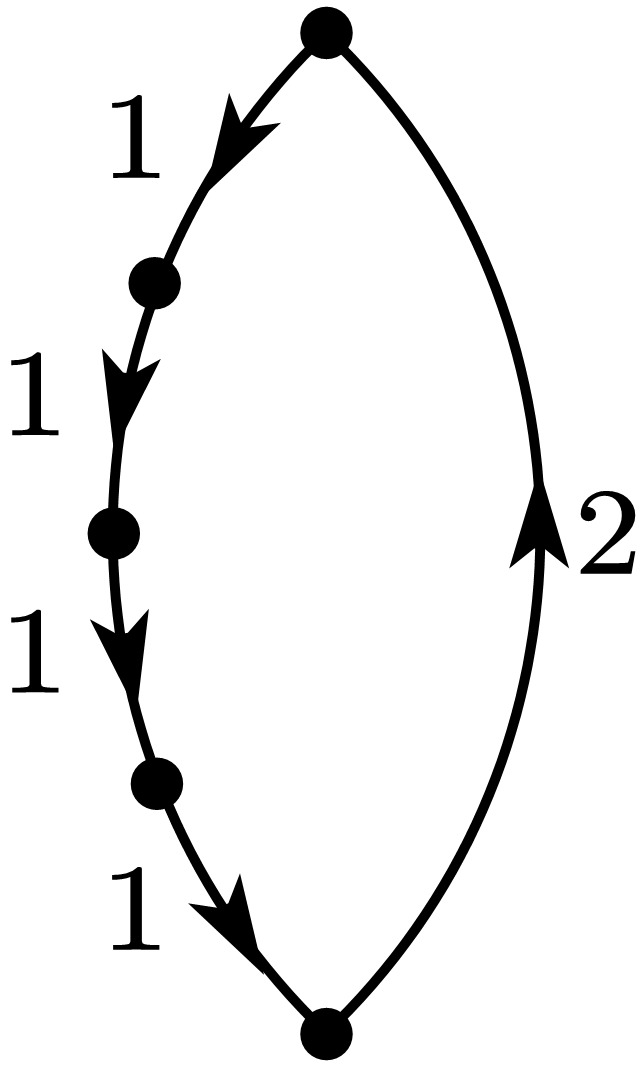
\includegraphics[scale=1.0,trim=0 -4 0 -4]{./pictures/6.01/1.png}
		\captionof*{figure}{$\displaystyle (-1)^{4+1} \frac{ V^3_{11} V_{12} V_{21} }{ ( E^{(0)}_1 - E^{(0)}_2)^4 }$}
		\end{minipage} &
		
		\begin{minipage}{0.22\linewidth}
		\centering
		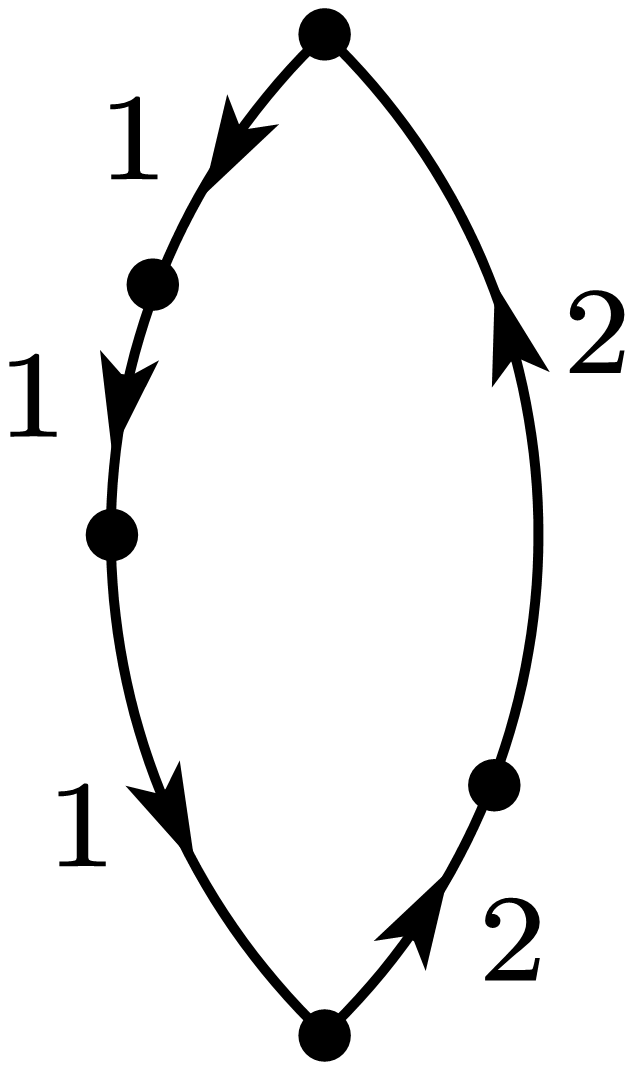
\includegraphics[scale=1.0,trim=0 -4 0 -4]{./pictures/6.01/2.png}
		\captionof*{figure}{$\displaystyle (-1)^{3+1} \frac{ V^2_{11} V_{12} V_{21} V_{22} }{ ( E^{(0)}_1 - E^{(0)}_2)^4 }$}
		\end{minipage} &
		
		\begin{minipage}{0.22\linewidth}
		\centering
		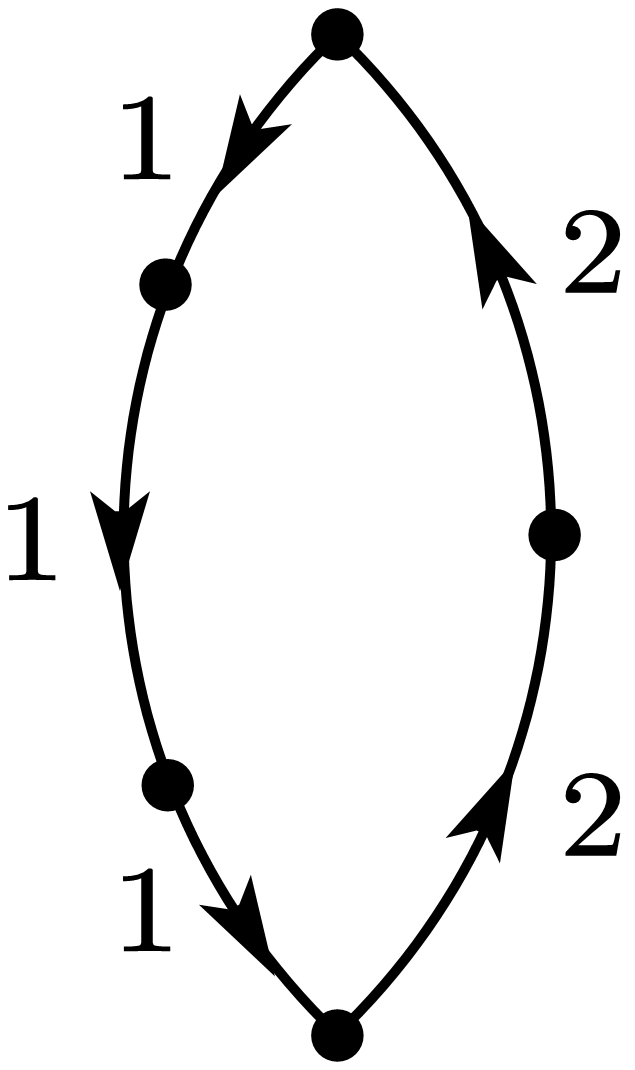
\includegraphics[scale=1.0,trim=0 -4 0 -4]{./pictures/6.01/3.png}
		\captionof*{figure}{$\displaystyle (-1)^{3+1} \frac{ V^2_{11} V_{12} V_{21} V_{22} }{ ( E^{(0)}_1 - E^{(0)}_2)^4 }$}
		\end{minipage} &
		
		\begin{minipage}{0.22\linewidth}
		\centering
		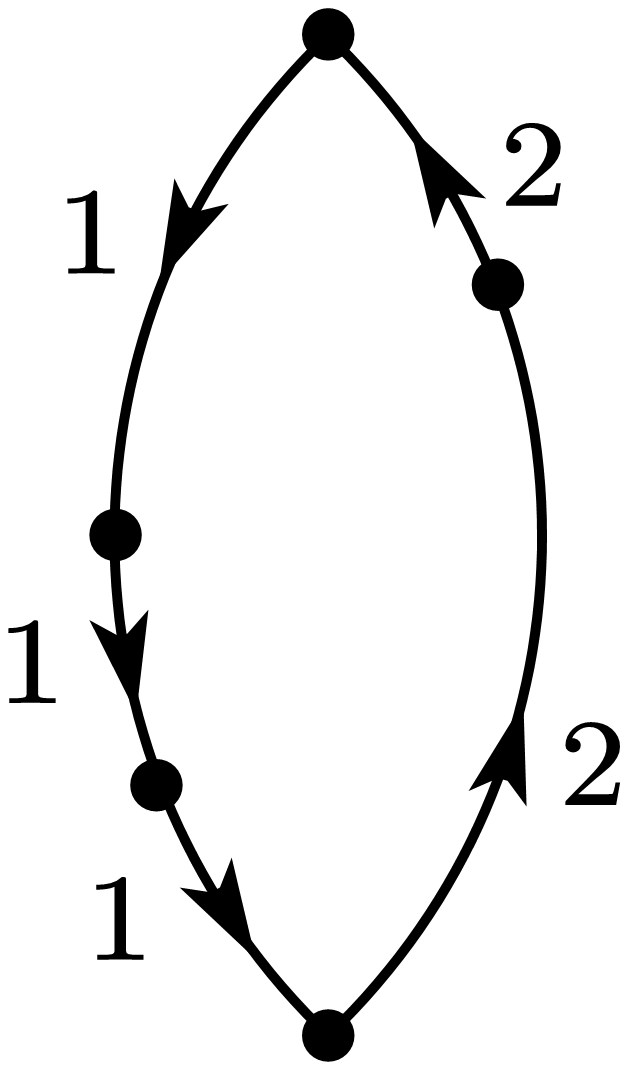
\includegraphics[scale=1.0,trim=0 -4 0 -4]{./pictures/6.01/4.png}
		\captionof*{figure}{$\displaystyle (-1)^{3+1} \frac{ V^2_{11} V_{12} V_{21} V_{22} }{ ( E^{(0)}_1 - E^{(0)}_2)^4 }$}
		\end{minipage} \\
			
		\begin{minipage}{0.22\linewidth}
		\centering
		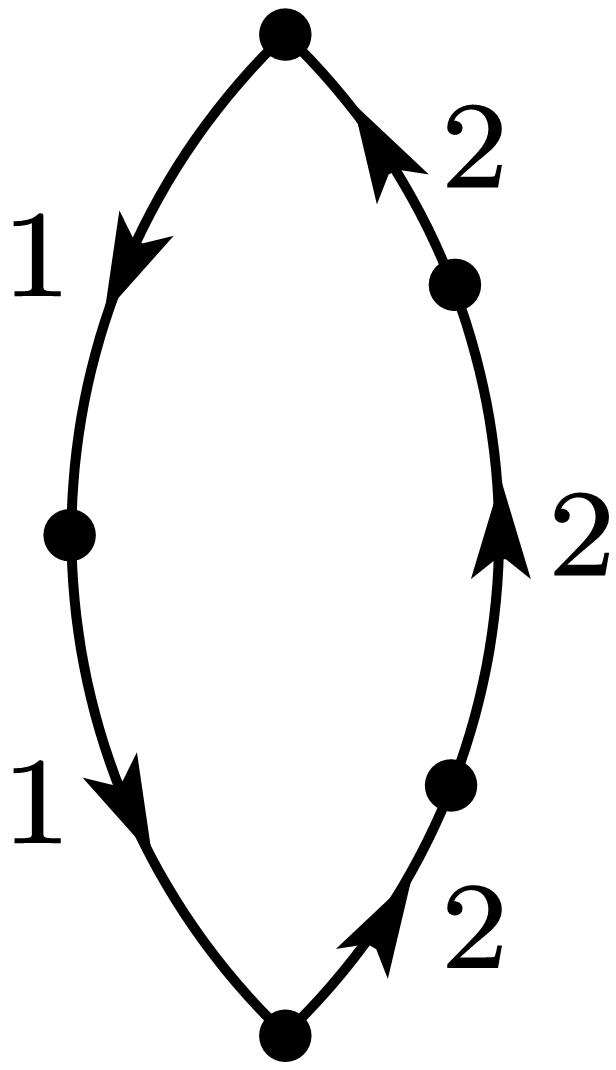
\includegraphics[scale=1.0,trim=0 -4 0 -4]{./pictures/6.01/5.png}
		\captionof*{figure}{$\displaystyle (-1)^{2+1} \frac{ V_{11} V_{12} V_{21} V^2_{22} }{ ( E^{(0)}_1 - E^{(0)}_2)^4 }$}
		\end{minipage} &
		
		\begin{minipage}{0.22\linewidth}
		\centering
		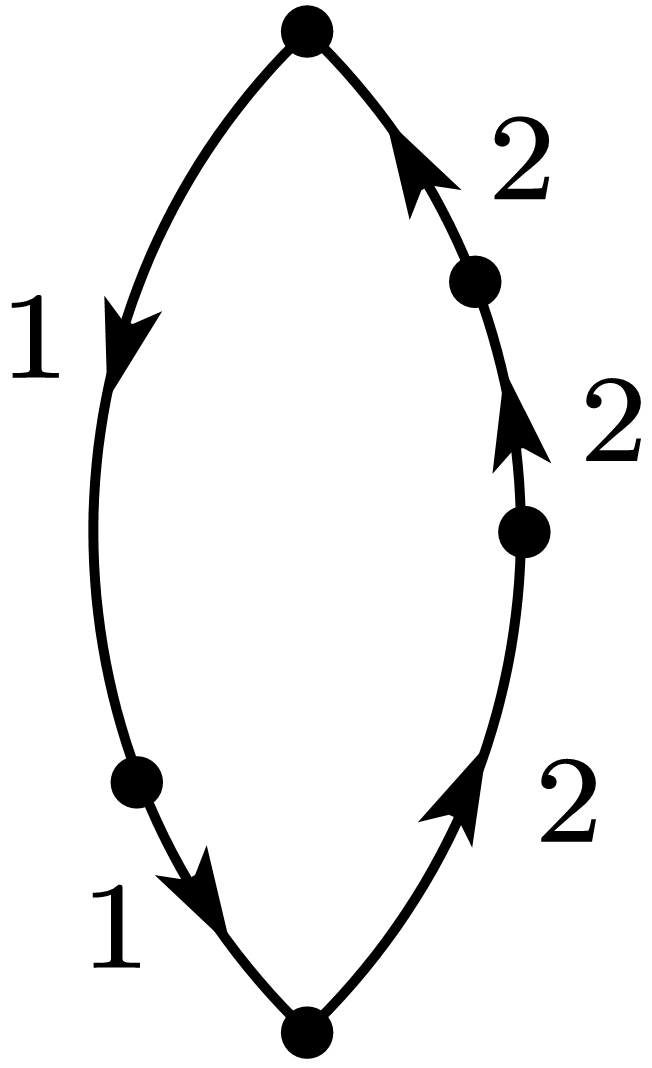
\includegraphics[scale=1.0,trim=0 -4 0 -4]{./pictures/6.01/6.png}
		\captionof*{figure}{$\displaystyle (-1)^{2+1} \frac{ V_{11} V_{12} V_{21} V^2_{22} }{ ( E^{(0)}_1 - E^{(0)}_2)^4 }$}
		\end{minipage} &
		
		\begin{minipage}{0.22\linewidth}
		\centering
		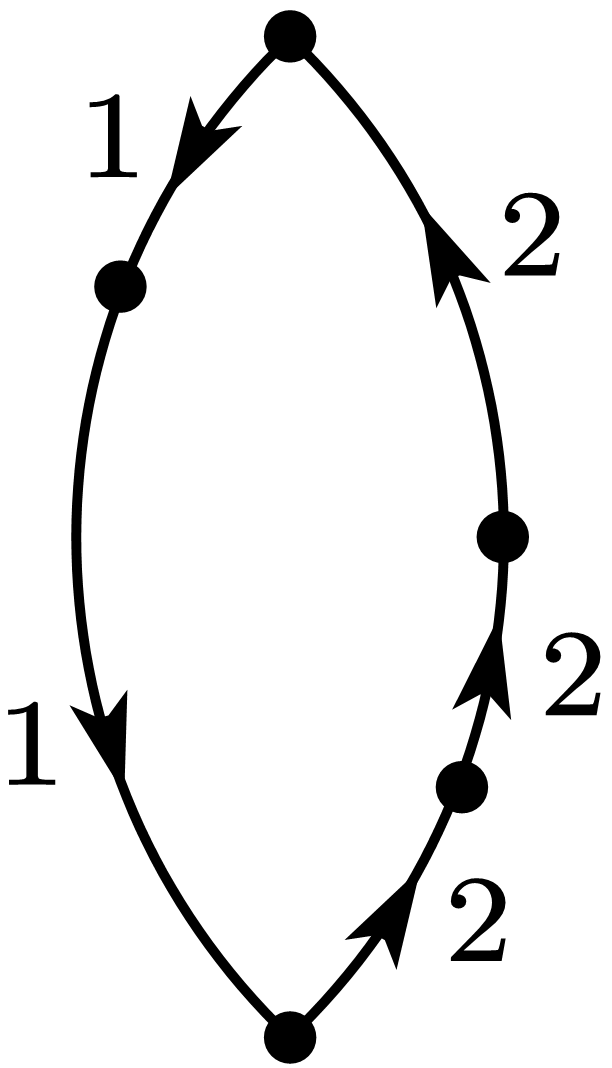
\includegraphics[scale=1.0,trim=0 -4 0 -4]{./pictures/6.01/7.png}
		\captionof*{figure}{$\displaystyle (-1)^{2+1} \frac{ V_{11} V_{12} V_{21} V^2_{22} }{ ( E^{(0)}_1 - E^{(0)}_2)^4 }$}
		\end{minipage} &
		
		\begin{minipage}{0.22\linewidth}
		\centering
		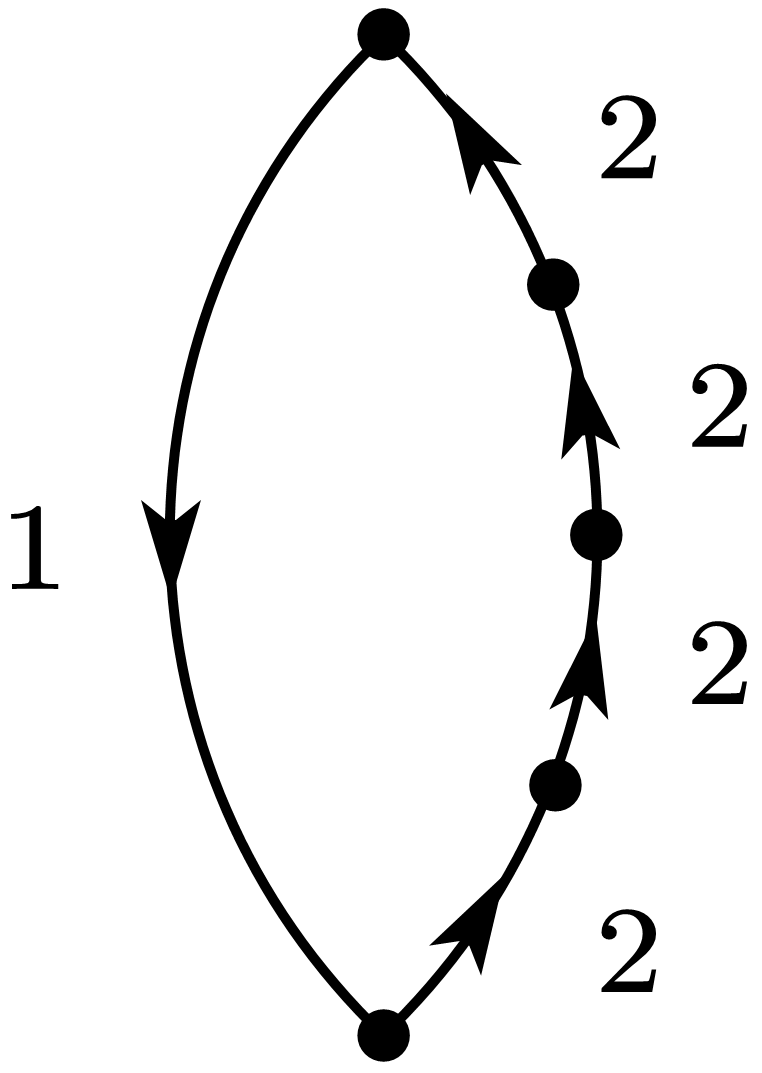
\includegraphics[scale=1.0,trim=0 -4 0 -4]{./pictures/6.01/8.png}
		\captionof*{figure}{$\displaystyle (-1)^{1+1} \frac{ V_{12} V_{21} V^3_{22} }{ ( E^{(0)}_1 - E^{(0)}_2)^4 }$}
		\end{minipage} 
		
	\end{tabular}
	\captionof{figure}{All fifth-order diagrams, which have the property that an imaginary horizontal line crosses only one hole and one particle line, and their mathematical expressions.}\label{fig:exe1}
	\end{center}
	
	Note that the diagrams, which have the property that an imaginary horizontal line crosses only one hole and one particle line, have no pair of hole/particle lines whose overlap is nonempty. For any pair of hole/particle lines which connect the dots $m_1$ and $n_1$, $m_2$ and $n_2$, where $n_1 > m_1$ and $n_2 > m_2$, their overlap will be 
	\begin{itemize}
	
	\item $[\max\{m_1, m_2\},\min\{n_1, n_2\}]$, if $\min\{n_1, n_2\} > \max\{m_1, m_2\}$;
	
	\item empty, otherwise. 
	
	\end{itemize}
	For example, if there is a pair of hole lines, one connecting the dot 1 and 3, and the other connecting 2 and 5, their overlap will be $[2, 3]$. Take an another example, if there is a pair of particle lines, one connecting the dot 5 and 4, and the other connecting 2 and 1, their overlap will be empty.
	
	Thus, there are four cases.
	\begin{itemize}
	
	\item Four hole lines and one particle line. There is only one method, hole lines are $(1,2)$, $(2,3)$, $(3,4)$, $(4,5)$ and the only particle line is $(5,1)$, as the first subdiagram in \Figref{fig:exe1}.
	
	\item Three hole lines and two particle lines. There are three methods as follows.
		\begin{itemize}
	
		\item Hole lines are $(1,2)$, $(2,3)$, and $(3,5)$ while particle lines are $(5,4)$, $(4,1)$.
		
		\item Hole lines are $(1,2)$, $(2,4)$, and $(4,5)$ while particle lines are $(5,3)$, $(3,1)$.
		
		\item Hole lines are $(1,3)$, $(3,4)$, and $(4,5)$ while particle lines are $(5,2)$, $(2,1)$.
	
		\end{itemize}
		They correspond to the second, third, fourth subdiagram in \Figref{fig:exe1}.
	
	\item Two hole lines and three particle lines. There are three methods as follows.
		\begin{itemize}
	
		\item Hole lines are $(1,3)$, $(3,5)$ while particle lines are $(5,4)$, $(4,2)$, and $(2,1)$.
		
		\item Hole lines are $(1,4)$, $(4,5)$ while particle lines are $(5,3)$, $(3,2)$, and $(2,1)$.
		
		\item Hole lines are $(1,2)$, $(2,5)$ while particle lines are $(5,4)$, $(4,3)$, and $(3,1)$.
	
		\end{itemize}
		They correspond to the fifth, sixth, seventh subdiagram in \Figref{fig:exe1}.
		
	\item One hole line and four particle lines. There is only one method, the only hole line is $(1,5)$ and particle lines are $(5,4)$, $(4,3)$, $(3,2)$, and $(2,1)$, as the eighth subdiagram in \Figref{fig:exe1}.
			
	\end{itemize}
	
	Thus, the sum of such diagrams is
	\begin{align*}
%		&\hspace{1.4em}(-1)^{4+1} \frac{ V^3_{11} V_{12} V_{21} }{ ( E^{(0)}_1 - E^{(0)}_2)^4 } + (-1)^{3+1} \frac{ V^2_{11} V_{12} V_{21} V_{22} }{ ( E^{(0)}_1 - E^{(0)}_2)^4 } + (-1)^{3+1} \frac{ V^2_{11} V_{12} V_{21} V_{22} }{ ( E^{(0)}_1 - E^{(0)}_2)^4 } \\
%		&\hspace{1.4em} + (-1)^{3+1} \frac{ V^2_{11} V_{12} V_{21} V_{22} }{ ( E^{(0)}_1 - E^{(0)}_2)^4 } + (-1)^{2+1} \frac{ V_{11} V_{12} V_{21} V^2_{22} }{ ( E^{(0)}_1 - E^{(0)}_2) }^4 + (-1)^{2+1} \frac{ V_{11} V_{12} V_{21} V^2_{22} }{ ( E^{(0)}_1 - E^{(0)}_2) }^4 \\
%		&\hspace{1.4em}  + (-1)^{2+1} \frac{ V_{11} V_{12} V_{21} V^2_{22} }{ ( E^{(0)}_1 - E^{(0)}_2) }^4 + (-1)^{1+1} \frac{ V_{12} V_{21} V^3_{22} }{ ( E^{(0)}_1 - E^{(0)}_2)^4 } \\
%		&= - \frac{ V^3_{11} V_{12} V_{21} }{ ( E^{(0)}_1 - E^{(0)}_2)^4 } + 3 \frac{ V^2_{11} V_{12} V_{21} V_{22} }{ ( E^{(0)}_1 - E^{(0)}_2)^4 } - 3 \frac{ V_{11} V_{12} V_{21} V^2_{22} }{ ( E^{(0)}_1 - E^{(0)}_2) }^4 + \frac{ V_{12} V_{21} V^3_{22} }{ ( E^{(0)}_1 - E^{(0)}_2)^4 } \\
%		&= 
		- \frac{ V_{12} V_{21} \left( V^3_{11} - 3 V^2_{11} V_{22} + 3 V_{11} V_{22} - V^3_{22} \right) }{ ( E^{(0)}_1 - E^{(0)}_2)^4 } = - \frac{ V_{12} V_{21} \left( V_{11} - V_{22} \right)^3 }{ ( E^{(0)}_1 - E^{(0)}_2)^4 } = \frac{ V_{12} V_{21} \left( V_{22} - V_{11} \right)^3 }{ ( E^{(0)}_1 - E^{(0)}_2)^4 }.
	\end{align*}
	
	In fact, as the textbook says, these eight diagrams can be generated by adding three dots to the second-order diagram in all positive ways. In fact, any pair of hole/particle lines in them has also empty overlap. I think the calculation of the overlap is much direct than inspecting the property of lines.
	
	\end{solution}

	\subsection{Diagrammatic Perturbation Theory for \texorpdfstring{$N$}- States}
	
	% 6.2
	\begin{exercise}
	Use diagrammatic techniques to obtain the fourth-order perturbation energy of a particular state (say, $i$) of an $N$-state system. That is, evaluate the diagrams
	\begin{center}
	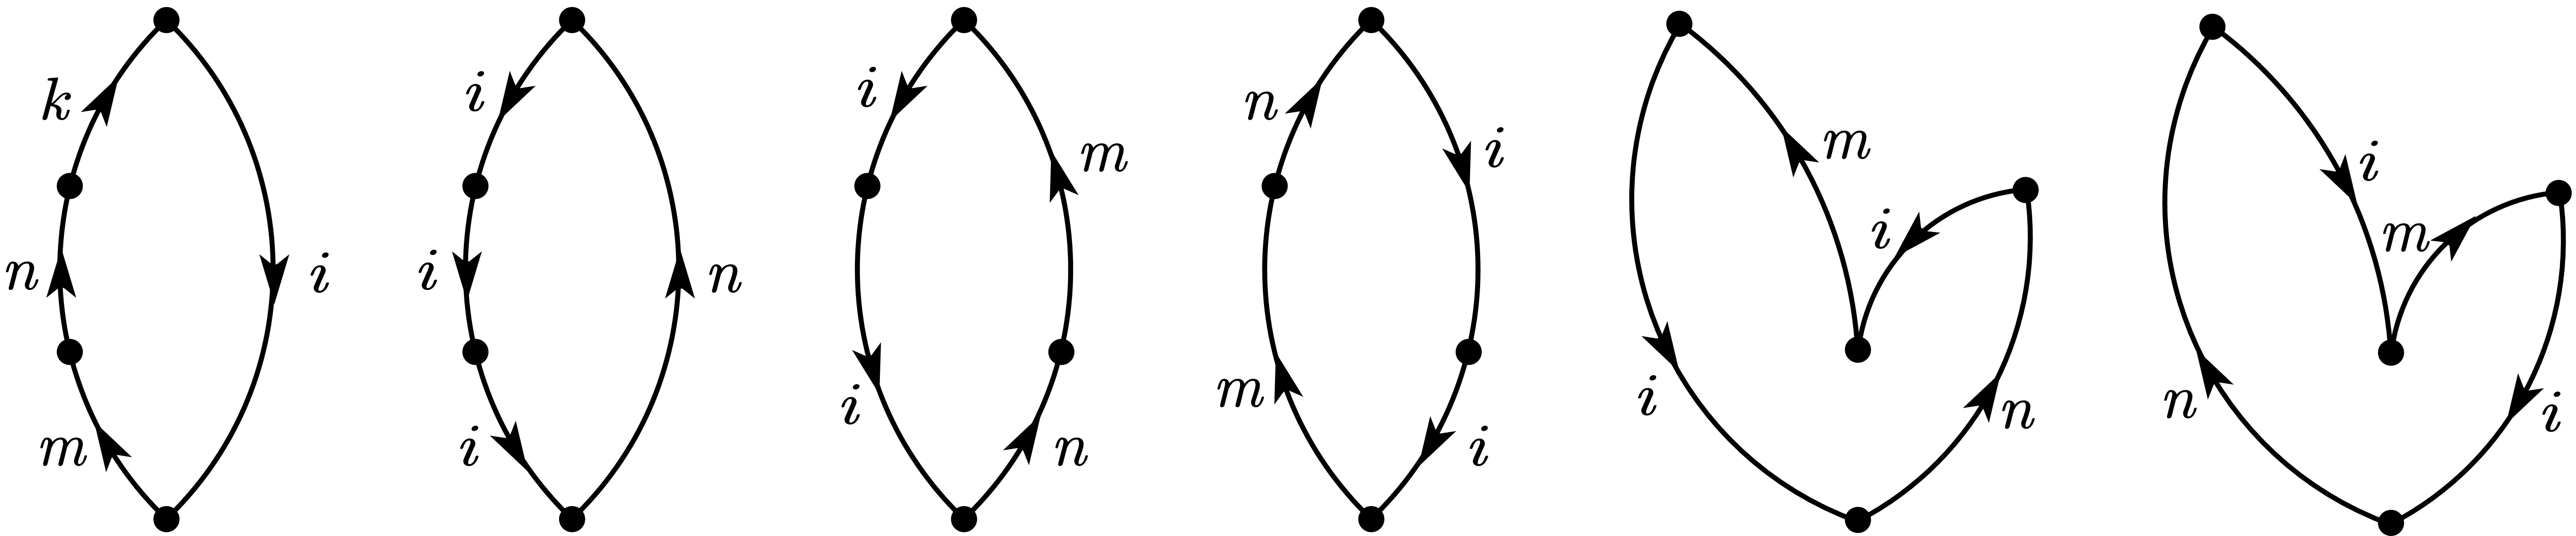
\includegraphics[scale=1.0]{./pictures/6.02/exercise.png}
	\end{center}
	where the indices $m$, $n$, $k$, ... exclude $i$. Using the approach of Section 6.1, obtain an algebraic expression for the fourth-order energy and compare it to the diagrammatic result.
	
	\end{exercise}
	
	\begin{solution}
	
	Firstly, all fourth-order diagrams and their mathematical expressions are listed in \Figref{fig:exe2}.
	
	\begin{center}
	\begin{tabular}{cc}
	
		\begin{minipage}{0.49\linewidth}
		\centering
		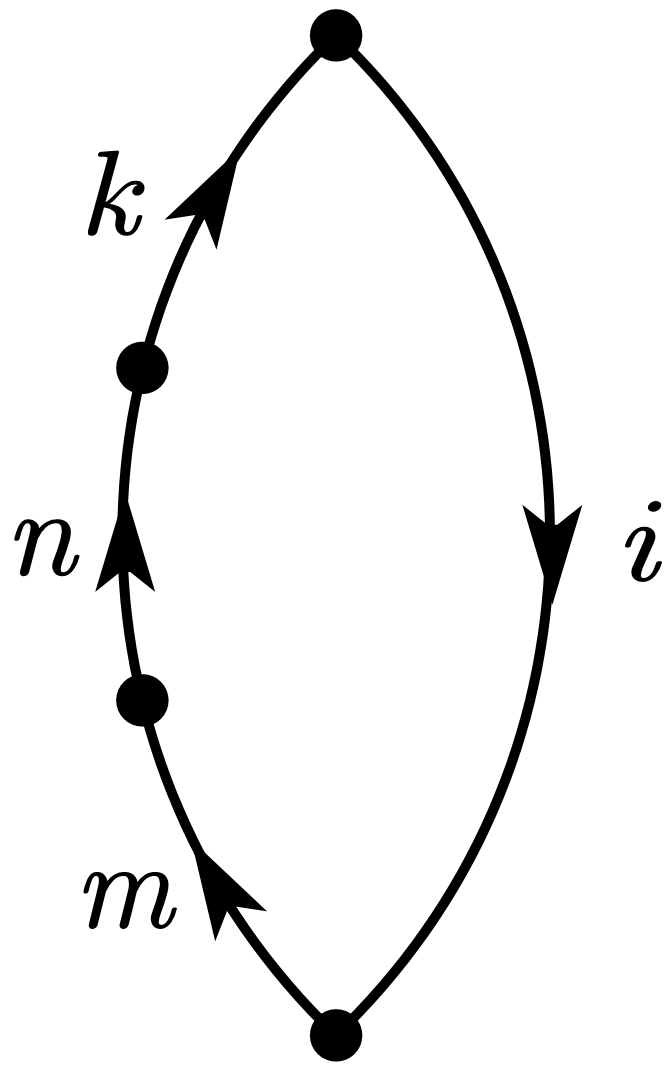
\includegraphics[scale=1.0,trim=0 -4 0 -4]{./pictures/6.02/1.png}
		\captionof*{figure}{$(-1)^{1+1} { \sum_{kmn} }^\prime \frac{ V_{ki} V_{nk} V_{mn} V_{im} }{ ( E^{(0)}_i - E^{(0)}_k ) ( E^{(0)}_i - E^{(0)}_n ) ( E^{(0)}_i - E^{(0)}_m ) }$}
		\end{minipage} &
		
		\begin{minipage}{0.42\linewidth}
		\centering
		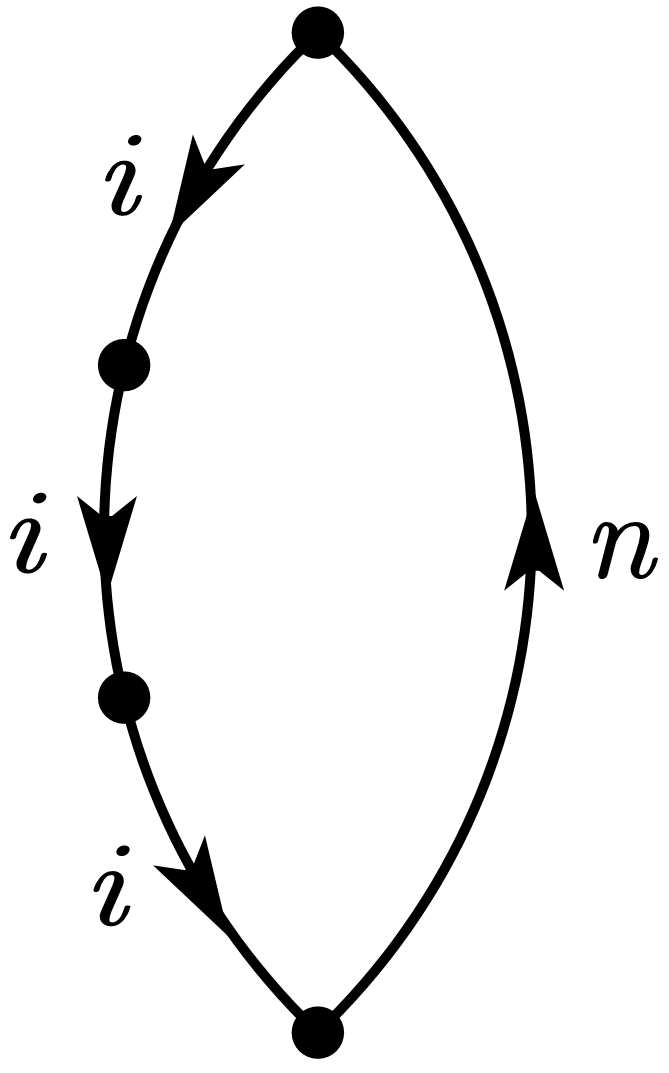
\includegraphics[scale=1.0,trim=0 -4 0 -4]{./pictures/6.02/2.png}
		\captionof*{figure}{$(-1)^{3+1} { \sum_n }^\prime \frac{ V_{ni} V^2_{ii} V_{in} }{ ( E^{(0)}_i - E^{(0)}_n)^3 }$}
		\end{minipage} \\
		
		\begin{minipage}{0.49\linewidth}
		\centering
		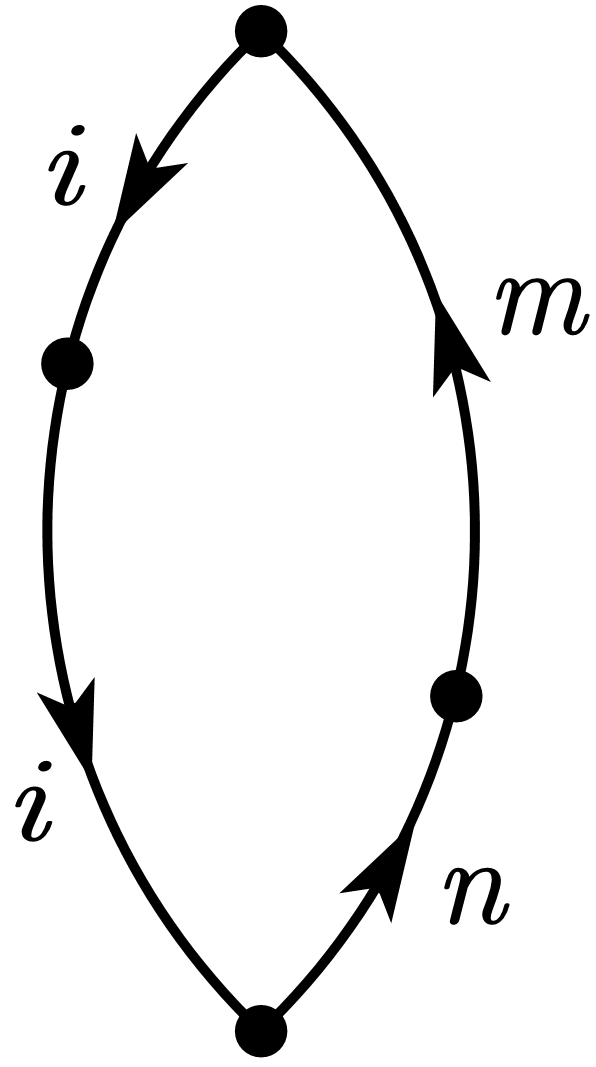
\includegraphics[scale=1.0,trim=0 -4 0 -4]{./pictures/6.02/3.png}
		\captionof*{figure}{$(-1)^{2+1} { \sum_{mn} }^\prime \frac{ V_{mi} V_{ii} V_{in} V_{nm} }{ ( E^{(0)}_i - E^{(0)}_n) ( E^{(0)}_i - E^{(0)}_m )^2 }$}
		\end{minipage}  &
			
		\begin{minipage}{0.42\linewidth}
		\centering
		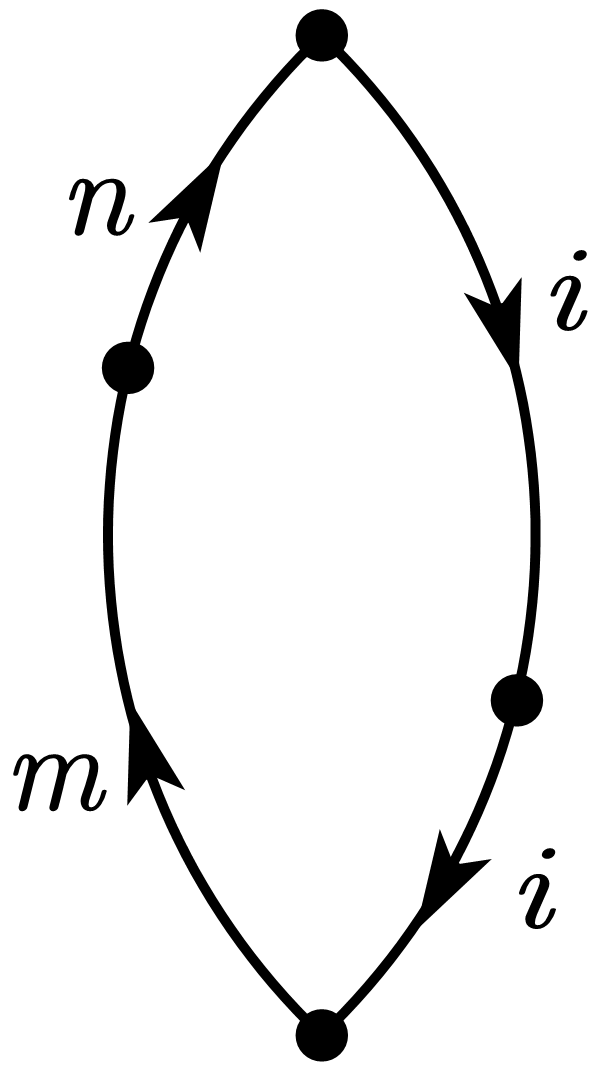
\includegraphics[scale=1.0,trim=0 -4 0 -4]{./pictures/6.02/4.png}
		\captionof*{figure}{$(-1)^{2+1} { \sum_{mn} }^\prime \frac{ V_{ni} V_{ii} V_{im} V_{mn} }{ ( E^{(0)}_i - E^{(0)}_n) ( E^{(0)}_i - E^{(0)}_m )^2 }$}
		\end{minipage} \\
		
		\begin{minipage}{0.49\linewidth}
		\centering
		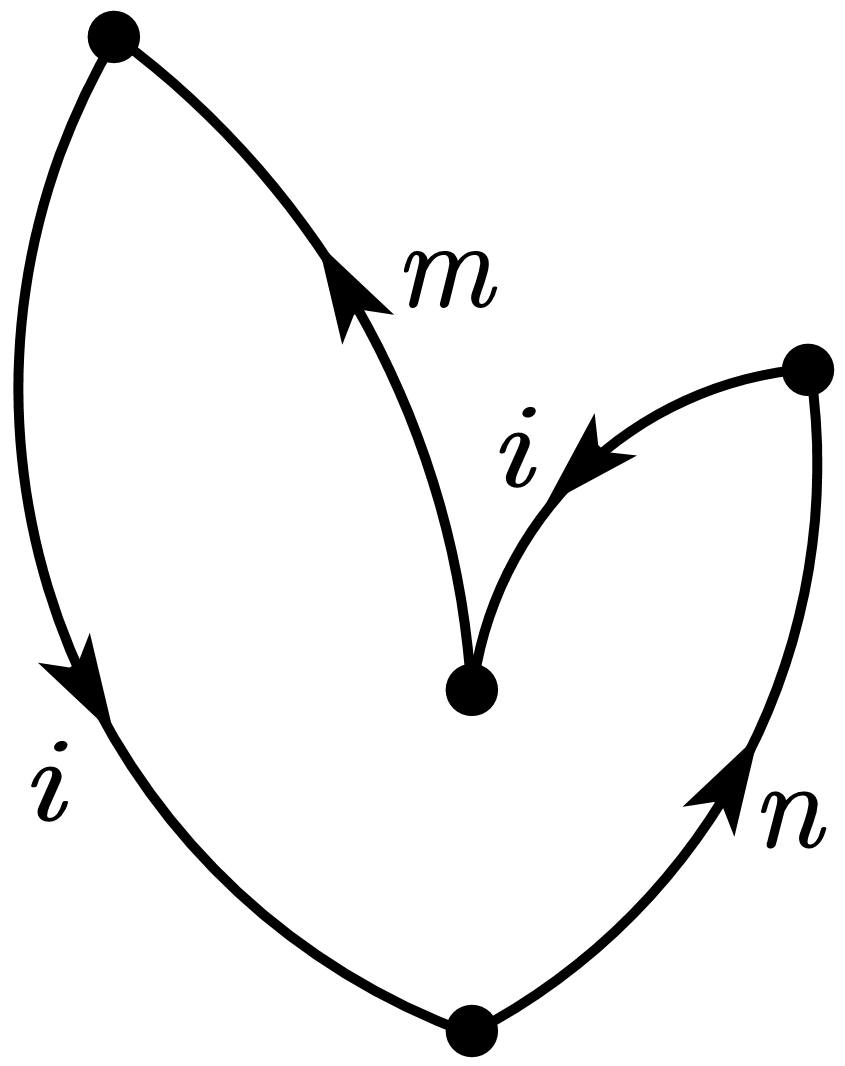
\includegraphics[scale=1.0,trim=0 -4 0 -4]{./pictures/6.02/5.png}
		\captionof*{figure}{$(-1)^{2+1} { \sum_{mn} }^\prime \frac{ V_{mi} V_{in} V_{ni} V_{im} }{ ( E^{(0)}_i - E^{(0)}_m ) ( 2E^{(0)}_i - E^{(0)}_m - E^{(0)}_n ) ( E^{(0)}_i - E^{(0)}_n ) }$}
		\end{minipage} &
		
		\begin{minipage}{0.42\linewidth}
		\centering
		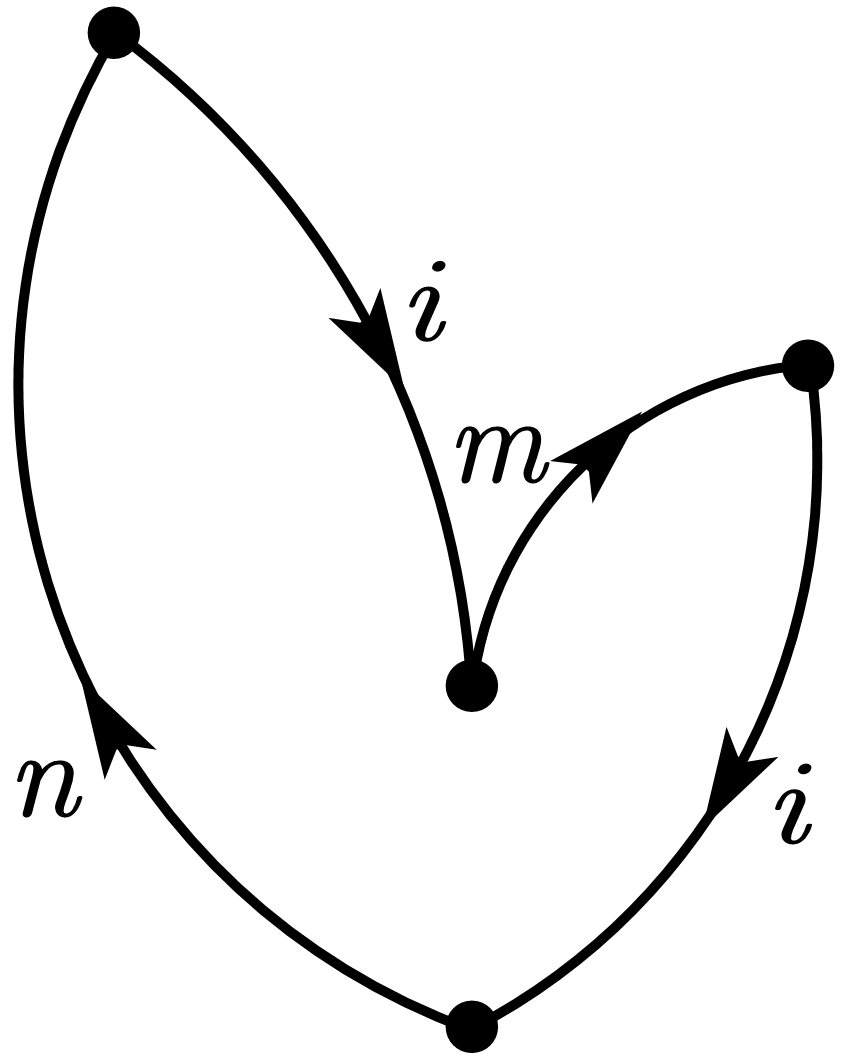
\includegraphics[scale=1.0,trim=0 -4 0 -4]{./pictures/6.02/6.png}
		\captionof*{figure}{$(-1)^{2+1} { \sum_{mn} }^\prime \frac{ V_{in} V_{ni} V_{im} V_{mi} }{ ( 2E^{(0)}_i - E^{(0)}_m - E^{(0)}_n ) ( E^{(0)}_i - E^{(0)}_n )^2 }$}
		\end{minipage} 
				
	\end{tabular}
	\captionof{figure}{All fourth-order diagrams and their mathematical expressions.}\label{fig:exe2}
	\end{center}
	
	Before the formal algebraic derivation, we should obtain some useful intermediate results. From (6.7d), multiplying by $\langle n |$, where $n \neq i$, we find that
	\[
		E^{(0)}_n \langle n | \Psi^{(3)}_i \rangle + \langle n | \mathscr{V} | \Psi^{(2)}_i \rangle = E^{(0)}_i \langle n | \Psi^{(3)}_i \rangle + E^{(1)}_i \langle n | \Psi^{(2)}_i \rangle + E^{(1)}_i \langle n | \Psi^{(2)}_i \rangle,
	\]
	and thus
	\[
		\langle n | \Psi^{(3)}_i \rangle = \frac{ 1 }{ E^{(0)}_i - E^{(0)}_n }\left[ \langle n | \mathscr{V} | \Psi^{(2)}_i \rangle - E^{(1)}_i \langle n | \Psi^{(2)}_i \rangle - E^{(1)}_i \langle n | \Psi^{(2)}_i \rangle \right].
	\]
	Moreover, (6.8b), (6.10), (6.12), and (6.14) are used in the formal derivation. The fourth-order perturbation energy $E^{(4)}_i$ can be divided into 3 terms, viz.,
	\begin{align*}
		E^{(4)}_i &= \langle i | \mathscr{V} | \Psi^{(3)}_i \rangle = { \sum_n }^\prime \langle i | \mathscr{V} | n \rangle \langle n | \Psi^{(3)}_i \rangle = { \sum_n }^\prime V_{in} \frac{ \langle n | \mathscr{V} | \Psi^{(2)}_i \rangle - E^{(1)}_i \langle n | \Psi^{(2)}_i \rangle - E^{(2)}_i \langle n | \Psi^{(1)}_i \rangle }{ E^{(0)}_i - E^{(0)}_n } \\
		&= { \sum_n }^\prime \frac{ V_{in} \langle n | \mathscr{V} | \Psi^{(2)}_i \rangle }{ E^{(0)}_i - E^{(0)}_n } - E^{(1)}_i { \sum_n }^\prime \frac{ V_{in} \langle n | \Psi^{(2)}_i \rangle }{ E^{(0)}_i - E^{(0)}_n } - E^{(2)}_i { \sum_n }^\prime \frac{ V_{in} \langle n | \Psi^{(1)}_i \rangle }{ E^{(0)}_i - E^{(0)}_n }.
	\end{align*}		
	The first term is
	\begin{align*}
		&\hspace{1.4em}{ \sum_n }^\prime \frac{ V_{in} \langle n | \mathscr{V} | \Psi^{(2)}_i \rangle }{ E^{(0)}_i - E^{(0)}_n } = { \sum_{mn} }^\prime \frac{ V_{in} \langle n | \mathscr{V} | m \rangle \langle m | \Psi^{(2)}_i \rangle }{ E^{(0)}_i - E^{(0)}_n } = { \sum_{mn} }^\prime \frac{ V_{in} V_{nm} }{ E^{(0)}_i - E^{(0)}_n } \langle m | \Psi^{(2)}_i \rangle \\
		&= { \sum_{mn} }^\prime \frac{ V_{in} V_{nm} }{ E^{(0)}_i - E^{(0)}_n } \frac{ \langle m | \mathscr{V} | \Psi^{(1)}_i \rangle - E^{(1)}_i \langle m | \Psi^{(1)}_i \rangle }{ E^{(0)}_i - E^{(0)}_m } \\
		&= { \sum_{mn} }^\prime \frac{ V_{in} V_{nm} }{ ( E^{(0)}_i - E^{(0)}_n )( E^{(0)}_i - E^{(0)}_m ) } \left[ \langle m | \mathscr{V} | \Psi^{(1)}_i \rangle - E^{(1)}_i \langle m | \Psi^{(1)}_i \rangle \right] \\
		&= { \sum_{mn} }^\prime \frac{ V_{in} V_{nm} }{ (E^{(0)}_i - E^{(0)}_n) (E^{(0)}_i - E^{(0)}_m) } \left[ { \sum_k }^\prime \langle m | \mathscr{V} | k \rangle \langle k | \Psi^{(1)}_i \rangle - E^{(1)}_i \langle m | \Psi^{(1)}_i \rangle \right] \\
		&= { \sum_{mnk} }^\prime \frac{ V_{in} V_{nm} V_{mk} }{ (E^{(0)}_i - E^{(0)}_n) (E^{(0)}_i - E^{(0)}_m) } \langle k | \Psi^{(1)}_i \rangle - { \sum_{mn} }^\prime \frac{ V_{ii} V_{in} V_{nm} }{ (E^{(0)}_i - E^{(0)}_n) (E^{(0)}_i - E^{(0)}_m) } \langle m | \Psi^{(1)}_i \rangle \\
		&= { \sum_{mnk} }^\prime \frac{ V_{in} V_{nm} V_{mk} }{ (E^{(0)}_i - E^{(0)}_n) (E^{(0)}_i - E^{(0)}_m) } \frac{ V_{ki} }{ E^{(0)}_i - E^{(0)}_k } - { \sum_{mn} }^\prime \frac{ V_{ii} V_{in} V_{nm} }{ (E^{(0)}_i - E^{(0)}_n) (E^{(0)}_i - E^{(0)}_m) } \frac{ V_{mi} }{ E^{(0)}_i - E^{(0)}_m } \\
		&= { \sum_{mnk} }^\prime \frac{ V_{in} V_{nm} V_{mk} V_{ki} }{ (E^{(0)}_i - E^{(0)}_n) (E^{(0)}_i - E^{(0)}_m) (E^{(0)}_i - E^{(0)}_k) } - { \sum_{mn} }^\prime \frac{ V_{ii} V_{in} V_{nm} V_{mi} }{ (E^{(0)}_i - E^{(0)}_n) (E^{(0)}_i - E^{(0)}_m)^2 } \\
		&= { \sum_{mnk} }^\prime \frac{ V_{im} V_{mn} V_{nk} V_{ki} }{ (E^{(0)}_i - E^{(0)}_n) (E^{(0)}_i - E^{(0)}_m) (E^{(0)}_i - E^{(0)}_k) } - { \sum_{mn} }^\prime \frac{ V_{ii} V_{in} V_{nm} V_{mi} }{ (E^{(0)}_i - E^{(0)}_n) (E^{(0)}_i - E^{(0)}_m)^2 }.
	\end{align*}
	It is evident that the first part of the first term correspond to the first subdiagram and the second part of the first term correspond to the third subdiagram.
	
	The second term is
	\begin{align*}
		&\hspace{1.4em}- E^{(1)}_i { \sum_n }^\prime \frac{ V_{in} \langle n | \Psi^{(2)}_i \rangle }{ E^{(0)}_i - E^{(0)}_n } - { \sum_n }^\prime \frac{ V_{ii} V_{in} }{ E^{(0)}_i - E^{(0)}_n } \langle n | \Psi^{(2)}_i \rangle \\
		&= - { \sum_n }^\prime \frac{ V_{ii} V_{in} }{ E^{(0)}_i - E^{(0)}_n } \frac{ \langle n | \mathscr{V} | \Psi^{(1)}_i \rangle - E^{(1)}_i \langle n | \Psi^{(1)}_i \rangle }{ E^{(0)}_i - E^{(0)}_n } \\
		&= - { \sum_n }^\prime \frac{ V_{ii} V_{in} }{ ( E^{(0)}_i - E^{(0)}_n )^2 } \langle n | \mathscr{V} | \Psi^{(1)}_i \rangle + E^{(1)}_i { \sum_n }^\prime \frac{ V_{ii} V_{in} }{ ( E^{(0)}_i - E^{(0)}_n )^2 } \langle n | \Psi^{(1)}_i \rangle \\
		&= - { \sum_n }^\prime \frac{ V_{ii} V_{in} }{ ( E^{(0)}_i - E^{(0)}_n )^2 } { \sum_m }^\prime \langle n | \mathscr{V} | m \rangle \langle m | \Psi^{(1)}_i \rangle + { \sum_n }^\prime \frac{ V^2_{ii} V_{in} }{ ( E^{(0)}_i - E^{(0)}_n )^2 } \langle n | \Psi^{(1)}_i \rangle \\
		&= - { \sum_{mn} }^\prime \frac{ V_{ii} V_{in} V_{nm} }{ ( E^{(0)}_i - E^{(0)}_n )^2 } \langle m | \Psi^{(1)}_i \rangle + { \sum_n }^\prime \frac{ V^2_{ii} V_{in} }{ ( E^{(0)}_i - E^{(0)}_n )^2 } \langle n | \Psi^{(1)}_i \rangle \\
		&= - { \sum_{mn} }^\prime \frac{ V_{ii} V_{in} V_{nm} }{ ( E^{(0)}_i - E^{(0)}_n )^2 } \frac{ \langle m | \mathscr{V} | i \rangle }{ E^{(0)}_i - E^{(0)}_m } + { \sum_n }^\prime \frac{ V^2_{ii} V_{in} }{ ( E^{(0)}_i - E^{(0)}_n )^2 } \frac{ \langle n | \mathscr{V} | i \rangle }{ E^{(0)}_i - E^{(0)}_n } \\
		&= - { \sum_{mn} }^\prime \frac{ V_{ii} V_{in} V_{nm} V_{mi} }{ ( E^{(0)}_i - E^{(0)}_n )^2 (E^{(0)}_i - E^{(0)}_m) } + { \sum_n }^\prime \frac{ V^2_{ii} V_{in} V_{ni} }{ ( E^{(0)}_i - E^{(0)}_n )^3 } \\
		&= - { \sum_{mn} }^\prime \frac{ V_{ii} V_{im} V_{mn} V_{ni} }{ ( E^{(0)}_i - E^{(0)}_m )^2 ( E^{(0)}_i - E^{(0)}_n ) } + { \sum_n }^\prime \frac{ V^2_{ii} V_{in} V_{ni} }{ ( E^{(0)}_i - E^{(0)}_n )^3 } .
	\end{align*}
	It is evident that the first part of the second term correspond to the fourth subdiagram and the second part of the second term correspond to the second subdiagram.
	
	The third term is
	\begin{align*}
		&\hspace{1.4em} -E^{(2)}_i { \sum_n }^\prime \frac{ V_{in} \langle n | \Psi^{(1)}_i \rangle }{ E^{(0)}_i - E^{(0)}_n } = -E^{(2)}_i { \sum_n }^\prime \frac{ V_{in} }{ E^{(0)}_i - E^{(0)}_n } \frac{ \langle n | \mathscr{V} | i \rangle }{ E^{(0)}_i - E^{(0)}_n } = -E^{(2)}_i { \sum_n }^\prime \frac{ V_{in} V_{ni} }{ ( E^{(0)}_i - E^{(0)}_n )^2 } \\
		&= - \left( { \sum_m }^\prime \frac{ V_{im} V_{mi} }{ ( E^{(0)}_i - E^{(0)}_m ) } \right) { \sum_n }^\prime \frac{ V_{in} V_{ni} }{ ( E^{(0)}_i - E^{(0)}_n )^2 } = - { \sum_{mn} }^\prime \frac{ V_{im} V_{mi} V_{in} V_{ni} }{ ( E^{(0)}_i - E^{(0)}_m )( E^{(0)}_i - E^{(0)}_n )^2 } .
	\end{align*}		
	
	It seems that it does not directly correspond to any subdiagram in \Figref{fig:exe2}. However, we can find that the sum of the mathematical expressions of the fifth and sixth subdiagram is
	\begin{align*}
		&\hspace{1.4em}(-1)^{2+1} { \sum_{mn} }^\prime \frac{ V_{mi} V_{in} V_{ni} V_{im} }{ ( E^{(0)}_i - E^{(0)}_m ) ( 2E^{(0)}_i - E^{(0)}_m - E^{(0)}_n ) ( E^{(0)}_i - E^{(0)}_n ) }  \\
		&\hspace{3.4em}+ (-1)^{2+1} { \sum_{mn} }^\prime \frac{ V_{in} V_{ni} V_{im} V_{mi} }{ ( 2E^{(0)}_i - E^{(0)}_m - E^{(0)}_n ) ( E^{(0)}_i - E^{(0)}_n )^2 } \\
		&= - { \sum_{mn} }^\prime \frac{ V_{in} V_{ni} V_{im} V_{mi} }{ ( 2E^{(0)}_i - E^{(0)}_m - E^{(0)}_n ) ( E^{(0)}_i - E^{(0)}_n ) } \left[ \frac{ 1 }{ E^{(0)}_i - E^{(0)}_m } + \frac{ 1 }{ E^{(0)}_i - E^{(0)}_n } \right] \\
		&= - { \sum_{mn} }^\prime \frac{ V_{in} V_{ni} V_{im} V_{mi} }{ ( 2E^{(0)}_i - E^{(0)}_m - E^{(0)}_n ) ( E^{(0)}_i - E^{(0)}_n ) } \frac{ 2E^{(0)}_i - E^{(0)}_m - E^{(0)}_n }{ ( E^{(0)}_i - E^{(0)}_m )( E^{(0)}_i - E^{(0)}_n ) } \\
		&= - { \sum_{mn} }^\prime \frac{ V_{im} V_{mi} V_{in} V_{ni} }{ ( E^{(0)}_i - E^{(0)}_m )( E^{(0)}_i - E^{(0)}_n )^2 } ,
	\end{align*}
	which is the third term exactly. Thus we can conclude that the results obtained by algebraic methods is the same as that by diagrammatic techniques. The mathematical expression of the fourth-order perturbation energy $E^{(4)}_i$ is
	\begin{align*}
		E^{(4)}_i &= { \sum_{mnk} }^\prime \frac{ V_{im} V_{mn} V_{nk} V_{ki} }{ (E^{(0)}_i - E^{(0)}_n) (E^{(0)}_i - E^{(0)}_m) (E^{(0)}_i - E^{(0)}_k) } - { \sum_{mn} }^\prime \frac{ V_{ii} V_{in} V_{nm} V_{mi} }{ (E^{(0)}_i - E^{(0)}_n) (E^{(0)}_i - E^{(0)}_m)^2 } \\
		&\hspace{2em} - { \sum_{mn} }^\prime \frac{ V_{ii} V_{im} V_{mn} V_{ni} }{ ( E^{(0)}_i - E^{(0)}_m )^2 ( E^{(0)}_i - E^{(0)}_n ) } + { \sum_n }^\prime \frac{ V^2_{ii} V_{in} V_{ni} }{ ( E^{(0)}_i - E^{(0)}_n )^3 } - { \sum_{mn} }^\prime \frac{ V_{im} V_{mi} V_{in} V_{ni} }{ ( E^{(0)}_i - E^{(0)}_m )( E^{(0)}_i - E^{(0)}_n )^2 } .
	\end{align*}
	
	\end{solution}
	
	\subsection{Summation of Diagrams}
	
	\section{Orbital Perturbation Theory: One-Particle Perturbations}	
	
	% 6.3	
	\begin{exercise}
	Derive
	\[
		E^{(2)}_0 = \sum_{ar} \frac{v_{ar}v_{ra}}{\varepsilon^{(0)}_a - \varepsilon^{(0)}_r}
	\]
	starting with the general expression for the second-order energy (Eq.(6.12)) applied to an $N$-electron system,
	\[
		E^{(2)}_0 = { \sum_n }^\prime \frac{\left| \langle \Psi_0 | \displaystyle\sum_i v(i)| n \rangle \right|^2 }{E^{(0)}_0-E^{(0)}_n}
	\]
	where the sum runs over all states of the system except the ground state.
	
	{\it Hint}: The states $| n \rangle$ must be single excitations of the type
	\[
		|\Psi^r_a\rangle = | \chi^{(0)}_1 \cdots \chi^{(0)}_{a-1} \chi^{(0)}_{r} \chi^{(0)}_{a+1} \cdots \chi^{(0)}_{N} \rangle.
	\]
	\end{exercise}
	
	\begin{solution}
	
	Note that (6.31) states that $\mathscr{V}=\sum_i v(i)$ only connects two Slater determinants whose different occupied orbitals should be no more than one, thus we obtain that
	\begin{sequation}
		E^{(2)}_0 = { \sum_n }^\prime \frac{\left| \langle \Psi_0 | \sum_i v(i)| n \rangle \right|^2 }{E^{(0)}_0-E^{(0)}_n} = \sum_{ ar } \frac{ \left| \langle \Psi_0 | \mathscr{V} | \Psi^r_a \rangle \right|^2 }{E^{(0)}_0-(E^{(0)}_0 + \varepsilon^{(0)}_r - \varepsilon^{(0)}_a) } = \sum_{ ar } \frac{ v_{ar} v_{ra} }{ \varepsilon^{(0)}_a - \varepsilon^{(0)}_r }.
	\end{sequation}
	
	\end{solution}
	
	% 6.4
	\begin{exercise}
	Calculate the third-order energy $E^{(3)}_0$ using the general expression given in Eq.(6.15).
	\begin{enumerate}
	
	\item[a.] Show that
	\[
		B^{(3)}_0 = - E^{(1)}_0 { \sum_n }^\prime \frac{|\langle \Psi_0 | \mathscr{V} | n \rangle |^2}{(E^{(0)}_0-E^{(0)}_n)^2} = - \sum_{abr} \frac{v_{aa} v_{rb} v_{br}}{( \varepsilon^{(0)}_b - \varepsilon^{(0)}_r)^2}.
	\]
		
	\item[b.] Show that
	\[
		A^{(3)}_0 = { \sum_{nm} }^\prime \frac{\langle \Psi_0 | \mathscr{V} | n \rangle \langle n | \mathscr{V} | m \rangle \langle m | \mathscr{V} | \Psi_0 \rangle}{(E^{(0)}_0-E^{(0)}_n)(E^{(0)}_0-E^{(0)}_m)} = \sum_{abrs} \frac{v_{ar} v_{sb} \langle \Psi^r_a | \mathscr{V} | \Psi^s_b \rangle}{( \varepsilon^{(0)}_a - \varepsilon^{(0)}_r)( \varepsilon^{(0)}_b - \varepsilon^{(0)}_s)}.
	\]
	
	\item[c.] Show that
	\begin{align*}
		\langle \Psi^r_a | \mathscr{V} | \Psi^s_b \rangle &= v_{rs} & \text{if} \, a = b  \quad r \neq s, \\
		&= - v_{ba} & \text{if} \, a \neq b \quad r = s, \\
		&= \sum_{c} v_{cc} - v_{aa} + v_{rr} & \text{if} \, a = b \quad r = s ,
	\end{align*}
	and zero otherwise.
		
	\item[d.] Finally, combine the two terms to obtain
	\[
		E^{(3)}_0 = A^{(3)}_0 + B^{(3)}_0 = \sum_{ars} \frac{v_{ar} v_{rs} v_{sa}}{( \varepsilon^{(0)}_a - \varepsilon^{(0)}_r)( \varepsilon^{(0)}_a - \varepsilon^{(0)}_s)} - \sum_{abr} \frac{v_{ra} v_{ab} v_{br}}{( \varepsilon^{(0)}_a - \varepsilon^{(0)}_r) ( \varepsilon^{(0)}_b - \varepsilon^{(0)}_r)}.
	\]
	
	\item[e.] Show that for a chosed-shell system
	\[
		E^{(3)}_0 = 2\sum_{ars}^{N/2} \frac{v_{ar} v_{rs} v_{sa}}{( \varepsilon^{(0)}_a - \varepsilon^{(0)}_r)( \varepsilon^{(0)}_a - \varepsilon^{(0)}_s)} - 2\sum_{abr}^{N/2} \frac{v_{ra} v_{ab} v_{br}}{( \varepsilon^{(0)}_a - \varepsilon^{(0)}_r) ( \varepsilon^{(0)}_b - \varepsilon^{(0)}_r)}.
	\]
	
	\end{enumerate}
	\end{exercise}
	
	\begin{solution}
	
	\begin{itemize}
	
	\item[a.] Similar to Exercise 6.3, it is evident that
	\begin{align*}
		B^{(3)}_0 &= - E^{(1)}_0 { \sum_n }^\prime \frac{|\langle \Psi_0 | \mathscr{V} | n \rangle |^2}{(E^{(0)}_0-E^{(0)}_n)^2} = - \left( \sum_{a} v_{aa} \right) \sum_{br} \frac{ v_{rb} v_{br}}{[ E^{(0)}_0- ( E^{(0)}_n + \varepsilon^{(0)}_r - \varepsilon^{(0)}_b ) ]^2} \\
		&= - \sum_{abr} \frac{ v_{aa} v_{rb} v_{br}}{( \varepsilon^{(0)}_b - \varepsilon^{(0)}_r)^2}.
	\end{align*}

	\item[b.] In the same way, we obtain that
	\begin{align*}
		A^{(3)}_0 &= { \sum_{nm} }^\prime \frac{\langle \Psi_0 | \mathscr{V} | n \rangle \langle n | \mathscr{V} | m \rangle \langle m | \mathscr{V} | \Psi_0 \rangle}{(E^{(0)}_0-E^{(0)}_n)(E^{(0)}_0-E^{(0)}_m)} \\
		&= \sum_{ar} \sum_{bs} \frac{\langle \Psi_0 | \mathscr{V} | \Psi^r_a \rangle \langle \Psi^r_a | \mathscr{V} | \Psi^s_b \rangle \langle \Psi^s_b | \mathscr{V} | \Psi_0 \rangle}{ [ E^{(0)}_0 - ( E^{(0)}_0 + \varepsilon^{(0)}_r - \varepsilon^{(0)}_a ) ][ E^{(0)}_0 - ( E^{(0)}_0 + \varepsilon^{(0)}_s - \varepsilon^{(0)}_b ) ]}  \\
		&= \sum_{abrs} \frac{v_{ar} v_{sb} \langle \Psi^r_a | \mathscr{V} | \Psi^s_b \rangle}{( \varepsilon^{(0)}_a - \varepsilon^{(0)}_r)( \varepsilon^{(0)}_b - \varepsilon^{(0)}_s)}.
	\end{align*}
	
	\item[c.] Using the conclusion of Exercise 2.13, at once we get
	\begin{align*}
		\langle \Psi^r_a | \mathscr{V} | \Psi^s_b \rangle &= v_{rs} & \text{if} \, a = b  \quad r \neq s, \\
		&= - v_{ba} & \text{if} \, a \neq b \quad r = s, \\
		&= \sum_{c} v_{cc} - v_{aa} + v_{rr} & \text{if} \, a = b \quad r = s ,
	\end{align*}
	and zero otherwise.
	
	\item[d.] Thus, we simplify $A^{(3)}_0$ as follows.
	\begin{align*}
		A^{(3)}_0 &= \sum_{abrs} \frac{ v_{ar} v_{sb} \langle \Psi^r_a | \mathscr{V} | \Psi^s_b \rangle}{ ( \varepsilon^{(0)}_a - \varepsilon^{(0)}_r) ( \varepsilon^{(0)}_b - \varepsilon^{(0)}_s) } \\
		&= \sum_{ar} \frac{ v_{ar} v_{ra} }{ ( \varepsilon^{(0)}_a - \varepsilon^{(0)}_r )^2} \left( \sum_{c} v_{cc} - v_{aa} + v_{rr} \right) + \sum_{ \substack{ar \\ s \neq r} } \frac{ v_{ar} v_{sa} v_{rs} }{ ( \varepsilon^{(0)}_a - \varepsilon^{(0)}_r)( \varepsilon^{(0)}_a - \varepsilon^{(0)}_s) } \\
		&\hspace{2em} + \sum_{ \substack{ar \\ b \neq a } } \frac{ v_{ar} v_{rb} ( - v_{ba} ) }{ ( \varepsilon^{(0)}_a - \varepsilon^{(0)}_r)( \varepsilon^{(0)}_b - \varepsilon^{(0)}_r) } \\
		&= \sum_{ar} \frac{ v_{ar} v_{ra} }{ ( \varepsilon^{(0)}_a - \varepsilon^{(0)}_r )^2} \left( \sum_{b} v_{bb} \right) - v_{aa} \sum_{ar} \frac{ v_{ar} v_{ra} }{ ( \varepsilon^{(0)}_a - \varepsilon^{(0)}_r )^2} + v_{rr} \sum_{ar} \frac{ v_{ar} v_{ra} }{ ( \varepsilon^{(0)}_a - \varepsilon^{(0)}_r )^2} \\
		&\hspace{2em} + \sum_{ \substack{ar \\ s \neq r} } \frac{ v_{ar} v_{sa} v_{rs} }{ ( \varepsilon^{(0)}_a - \varepsilon^{(0)}_r)( \varepsilon^{(0)}_a - \varepsilon^{(0)}_s) } - \sum_{ \substack{ar \\ b \neq a } } \frac{ v_{ar} v_{rb} v_{ba} }{ ( \varepsilon^{(0)}_a - \varepsilon^{(0)}_r)( \varepsilon^{(0)}_b - \varepsilon^{(0)}_r) } \\
		&= \left( \sum_{a} v_{aa} \right) \sum_{br} \frac{ v_{br} v_{rb} }{ ( \varepsilon^{(0)}_b - \varepsilon^{(0)}_r )^2} + \sum_{ ars } \frac{ v_{ar} v_{sa} v_{rs} }{ ( \varepsilon^{(0)}_a - \varepsilon^{(0)}_r)( \varepsilon^{(0)}_a - \varepsilon^{(0)}_s) } - \sum_{ abr } \frac{ v_{ar} v_{rb} v_{ba} }{ ( \varepsilon^{(0)}_a - \varepsilon^{(0)}_r)( \varepsilon^{(0)}_b - \varepsilon^{(0)}_r) } \\
		&= \sum_{abr} \frac{ v_{aa} v_{br} v_{rb} }{ ( \varepsilon^{(0)}_b - \varepsilon^{(0)}_r )^2} + \sum_{ ars } \frac{ v_{ar} v_{sa} v_{rs} }{ ( \varepsilon^{(0)}_a - \varepsilon^{(0)}_r)( \varepsilon^{(0)}_a - \varepsilon^{(0)}_s) } - \sum_{ abr } \frac{ v_{ar} v_{rb} v_{ba} }{ ( \varepsilon^{(0)}_a - \varepsilon^{(0)}_r)( \varepsilon^{(0)}_b - \varepsilon^{(0)}_r) } .
	\end{align*}
	Finally,
	\begin{align*}
		E^{(3)}_0 &= A^{(3)}_0 + B^{(3)}_0 \\
		&= \sum_{abr} \frac{ v_{aa} v_{br} v_{rb} }{ ( \varepsilon^{(0)}_b - \varepsilon^{(0)}_r )^2} + \sum_{ ars } \frac{ v_{ar} v_{sa} v_{rs} }{ ( \varepsilon^{(0)}_a - \varepsilon^{(0)}_r)( \varepsilon^{(0)}_a - \varepsilon^{(0)}_s) } \\
		&\hspace{2em} - \sum_{ abr } \frac{ v_{ar} v_{rb} v_{ba} }{ ( \varepsilon^{(0)}_a - \varepsilon^{(0)}_r)( \varepsilon^{(0)}_b - \varepsilon^{(0)}_r) } - \sum_{abr} \frac{ v_{aa} v_{rb} v_{br}}{( \varepsilon^{(0)}_b - \varepsilon^{(0)}_r)^2} \\
		&= \sum_{ ars } \frac{ v_{ar} v_{sa} v_{rs} }{ ( \varepsilon^{(0)}_a - \varepsilon^{(0)}_r)( \varepsilon^{(0)}_a - \varepsilon^{(0)}_s) } - \sum_{ abr } \frac{ v_{br} v_{ra} v_{ab} }{ ( \varepsilon^{(0)}_a - \varepsilon^{(0)}_r)( \varepsilon^{(0)}_b - \varepsilon^{(0)}_r) } .
	\end{align*}
	
	\item[e.] Since a matrix element $v_{ij}=\langle i | v | j \rangle$ is nonzero only if both spin orbitals $i$ and $j$ have the same spin, thus only $v_{ar} v_{sa} v_{rs}$ and $v_{\bar{a}\bar{r}} v_{\bar{s} \bar{a}} v_{\bar{r} \bar{s}}$ contribute, and so $v_{br} v_{ra} v_{ab}$ and $v_{\bar{b}\bar{r}} v_{\bar{r} \bar{a}} v_{\bar{a} \bar{b}}$ do $v_{br} v_{ra} v_{ab}$. Besides, the denominators is invariant regardless of spin up or down. In this way, we obtain that
	\begin{align*}
		E^{(3)}_0 &= \sum_{ ars }^{N/2} \frac{ v_{ar} v_{sa} v_{rs} }{ ( \varepsilon^{(0)}_a - \varepsilon^{(0)}_r)( \varepsilon^{(0)}_a - \varepsilon^{(0)}_s) } + \sum_{ \bar{a} \bar{r} \bar{s} }^{N/2} \frac{ v_{\bar{a} \bar{r}} v_{\bar{s} \bar{a} } v_{ \bar{r} \bar{s}} }{ ( \varepsilon^{(0)}_{\bar{a}} - \varepsilon^{(0)}_{\bar{r}})( \varepsilon^{(0)}_{\bar{a}} - \varepsilon^{(0)}_{\bar{s}}) } \\
		&\hspace{2em} - \sum_{ abr }^{N/2} \frac{ v_{br} v_{ra} v_{ab} }{ ( \varepsilon^{(0)}_a - \varepsilon^{(0)}_r)( \varepsilon^{(0)}_b - \varepsilon^{(0)}_r) } - \sum_{ \bar{a} \bar{b} \bar{r} }^{N/2} \frac{ v_{\bar{b} \bar{r}} v_{\bar{r} \bar{a}} v_{\bar{a} \bar{b} } }{ ( \varepsilon^{(0)}_{\bar{a}} - \varepsilon^{(0)}_{\bar{r}})( \varepsilon^{(0)}_{\bar{b}} - \varepsilon^{(0)}_{\bar{r}}) } \\
		&= 2 \sum_{ ars }^{N/2} \frac{ v_{ar} v_{sa} v_{rs} }{ ( \varepsilon^{(0)}_a - \varepsilon^{(0)}_r)( \varepsilon^{(0)}_a - \varepsilon^{(0)}_s) } - 2 \sum_{ abr }^{N/2} \frac{ v_{br} v_{ra} v_{ab} }{ ( \varepsilon^{(0)}_a - \varepsilon^{(0)}_r)( \varepsilon^{(0)}_b - \varepsilon^{(0)}_r) }.
	\end{align*}
	
	\end{itemize}		
	
	\end{solution}
	
	% 6.5
	\begin{exercise}
	Show that the second term in Eq.(6.52) is equal to $\frac{3}{8}\beta$ for benzene.
	\end{exercise}
	
	\begin{solution}
	
	The pictorial representation of the second term in $E^{(3)}_0$ can be seen in \Figref{fig:exe5}. 
	\begin{center}
		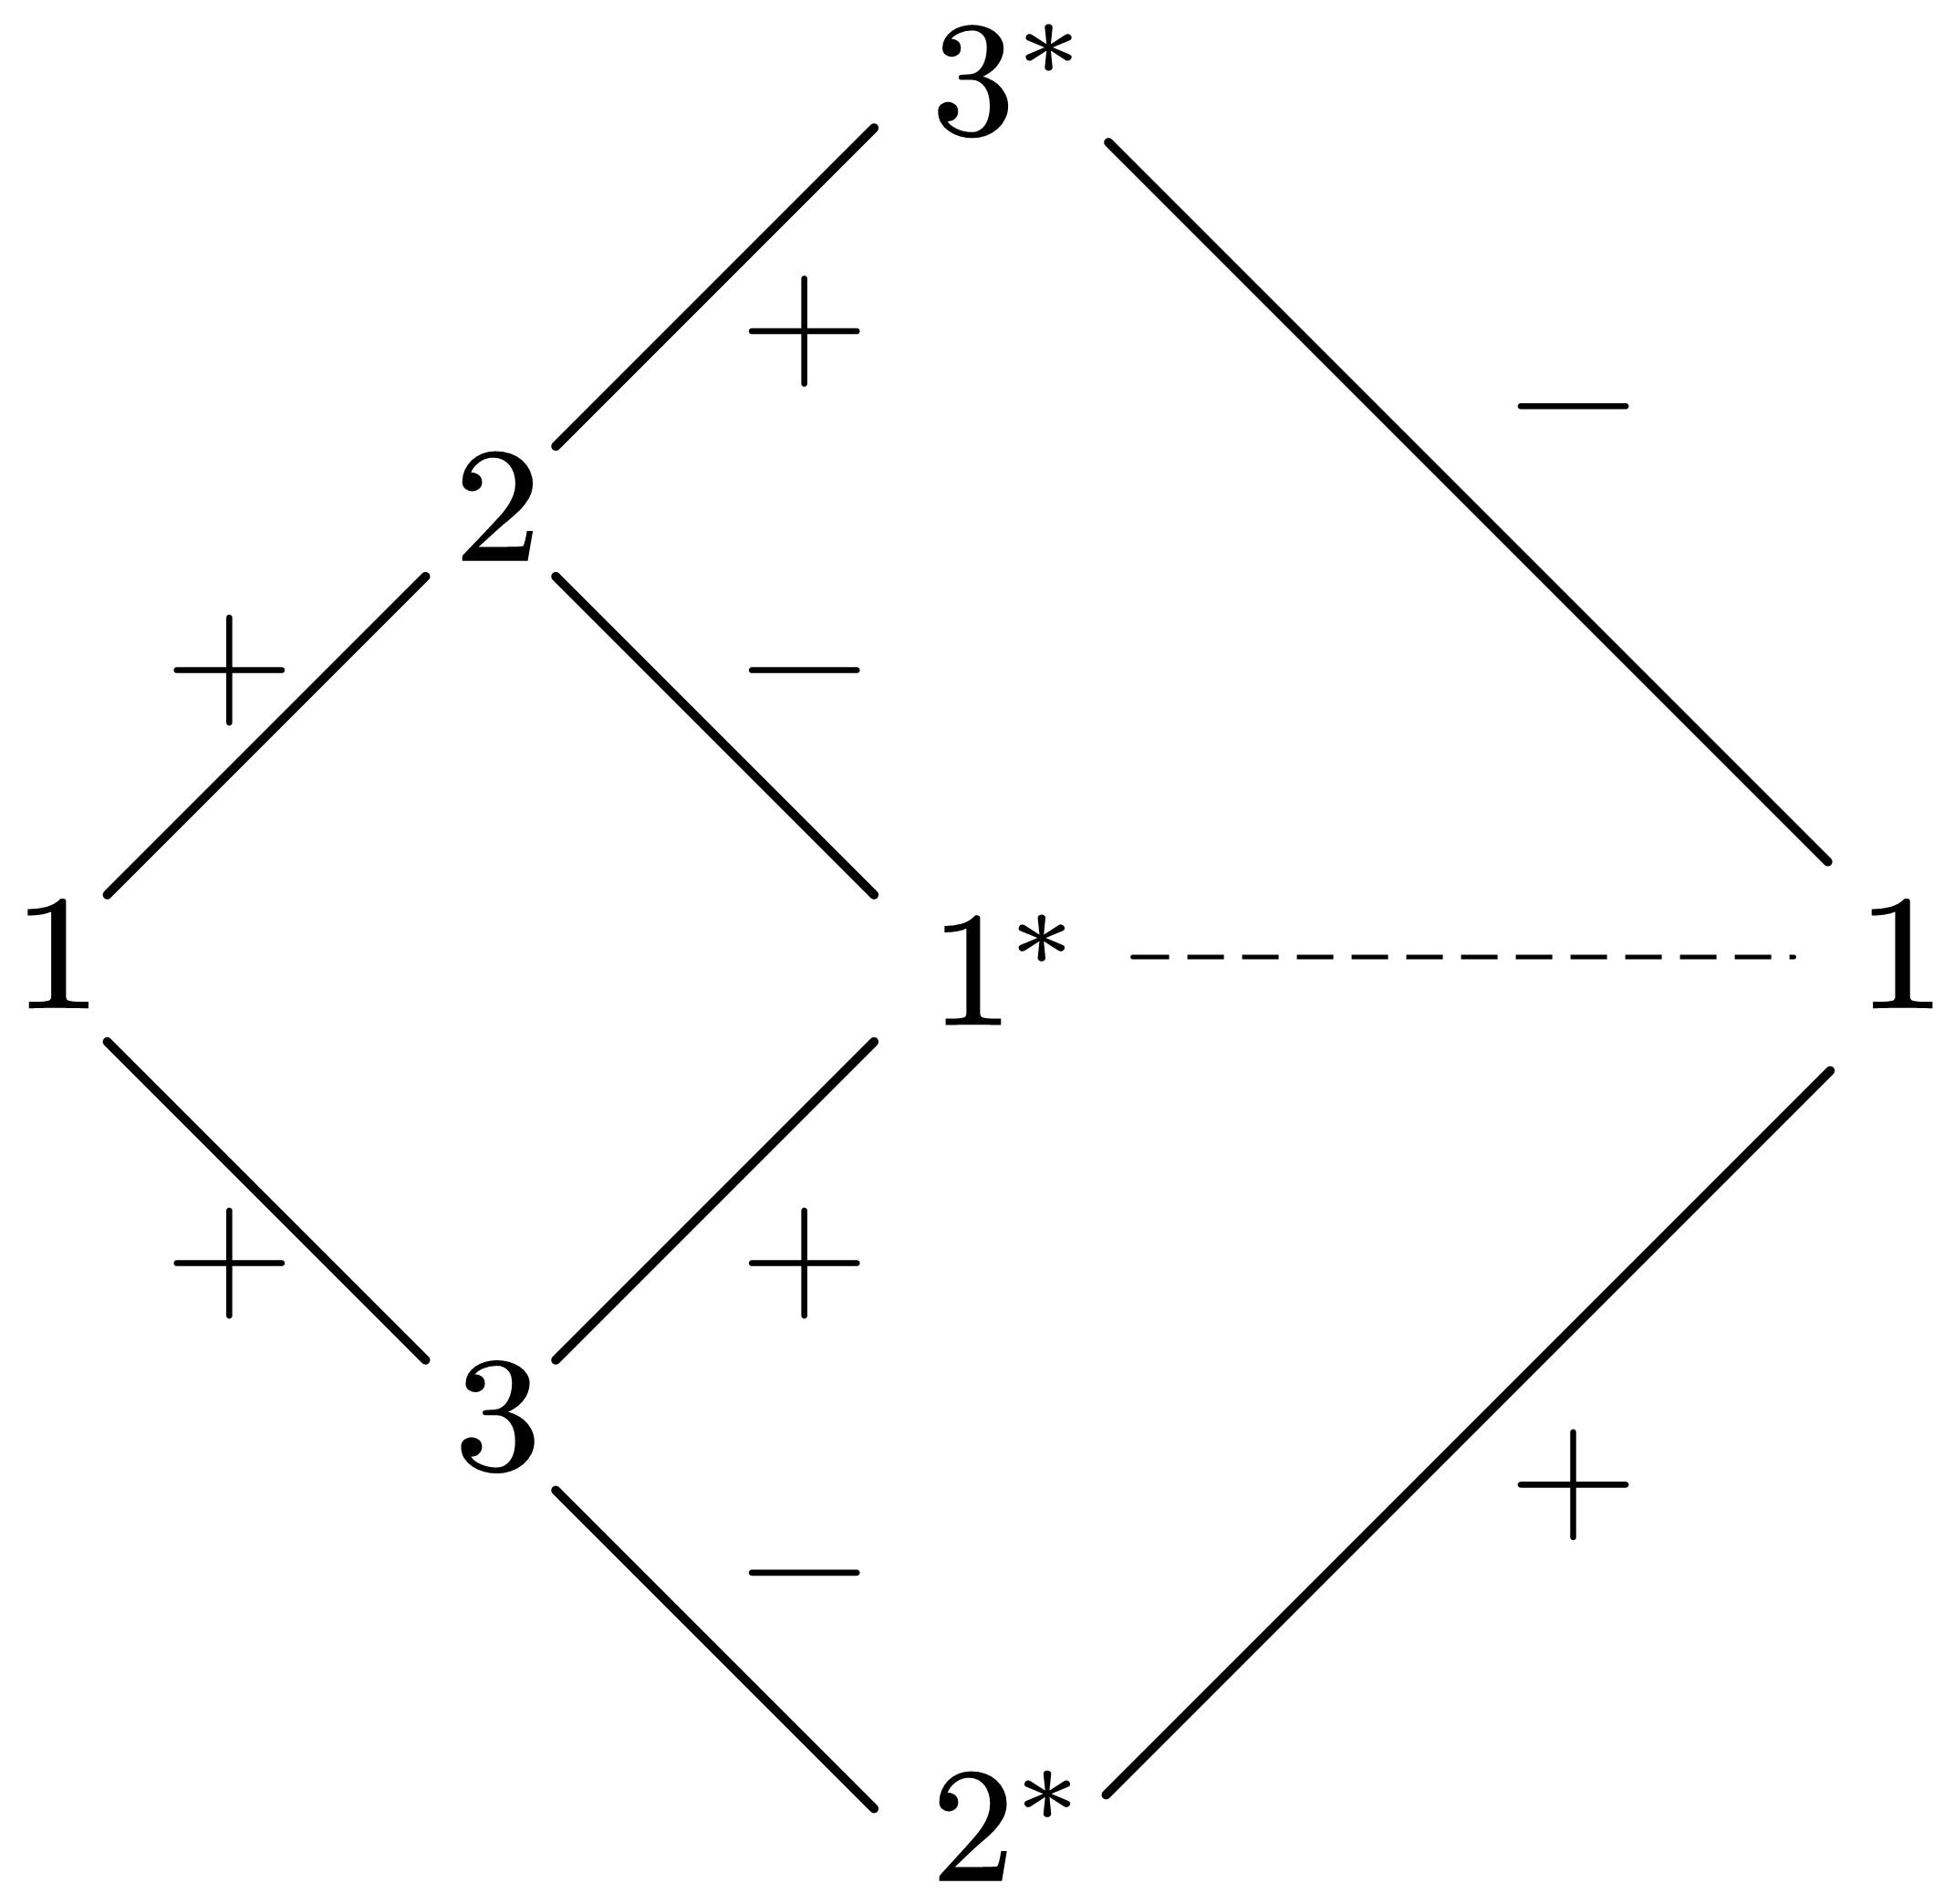
\includegraphics[scale=0.8]{./pictures/6.05/pictorial_representation_1.png}
		\captionof{figure}{Pictorial representation of the second term in $E^{(3)}_0$, where the order is $v_{ij}$, $v_{jk^*}$ and $v_{k^*i}$ from the left to the right. The plus and minus signs indicate whether the matrix elements between the two orbitals is $\pm \frac{\beta}{2}$.}\label{fig:exe5}
	\end{center}
	
	With the high symmetry, it is
	\begin{sequation}
		-2 \times \frac{1}{ (2\beta)^2 } \sum_{i=1}^3 \left[ v_{12} v_{23^*} v_{3^*1} + v_{13} v_{32^*} v_{2^*1} \right] = - \frac{3}{ 2\beta^2 } \left[ \frac{ \beta }{2} \times \frac{ \beta }{2} \times \left( - \frac{ \beta }{2} \right) + \frac{ \beta }{2} \times \left( - \frac{ \beta }{2} \right) \times \frac{ \beta }{2} \right] = \frac{3}{8\beta} .
	\end{sequation}	
	
	\end{solution}

	% 6.6
		\begin{exercise}
	Consider a cyclic polyene with $N = 4\nu+2$, $\nu=1$, $2$, ... carbons. Instead of assuming that all the bonds are identical, suppose they alternate in length. In the context of H{\"u}ckel theory this means that the resonance integrals between adjacent carbons are not all equal to $\beta$ but alternate between $\beta_11$ and $\beta_2$. For example, for benzene we have
	
	\begin{center}
	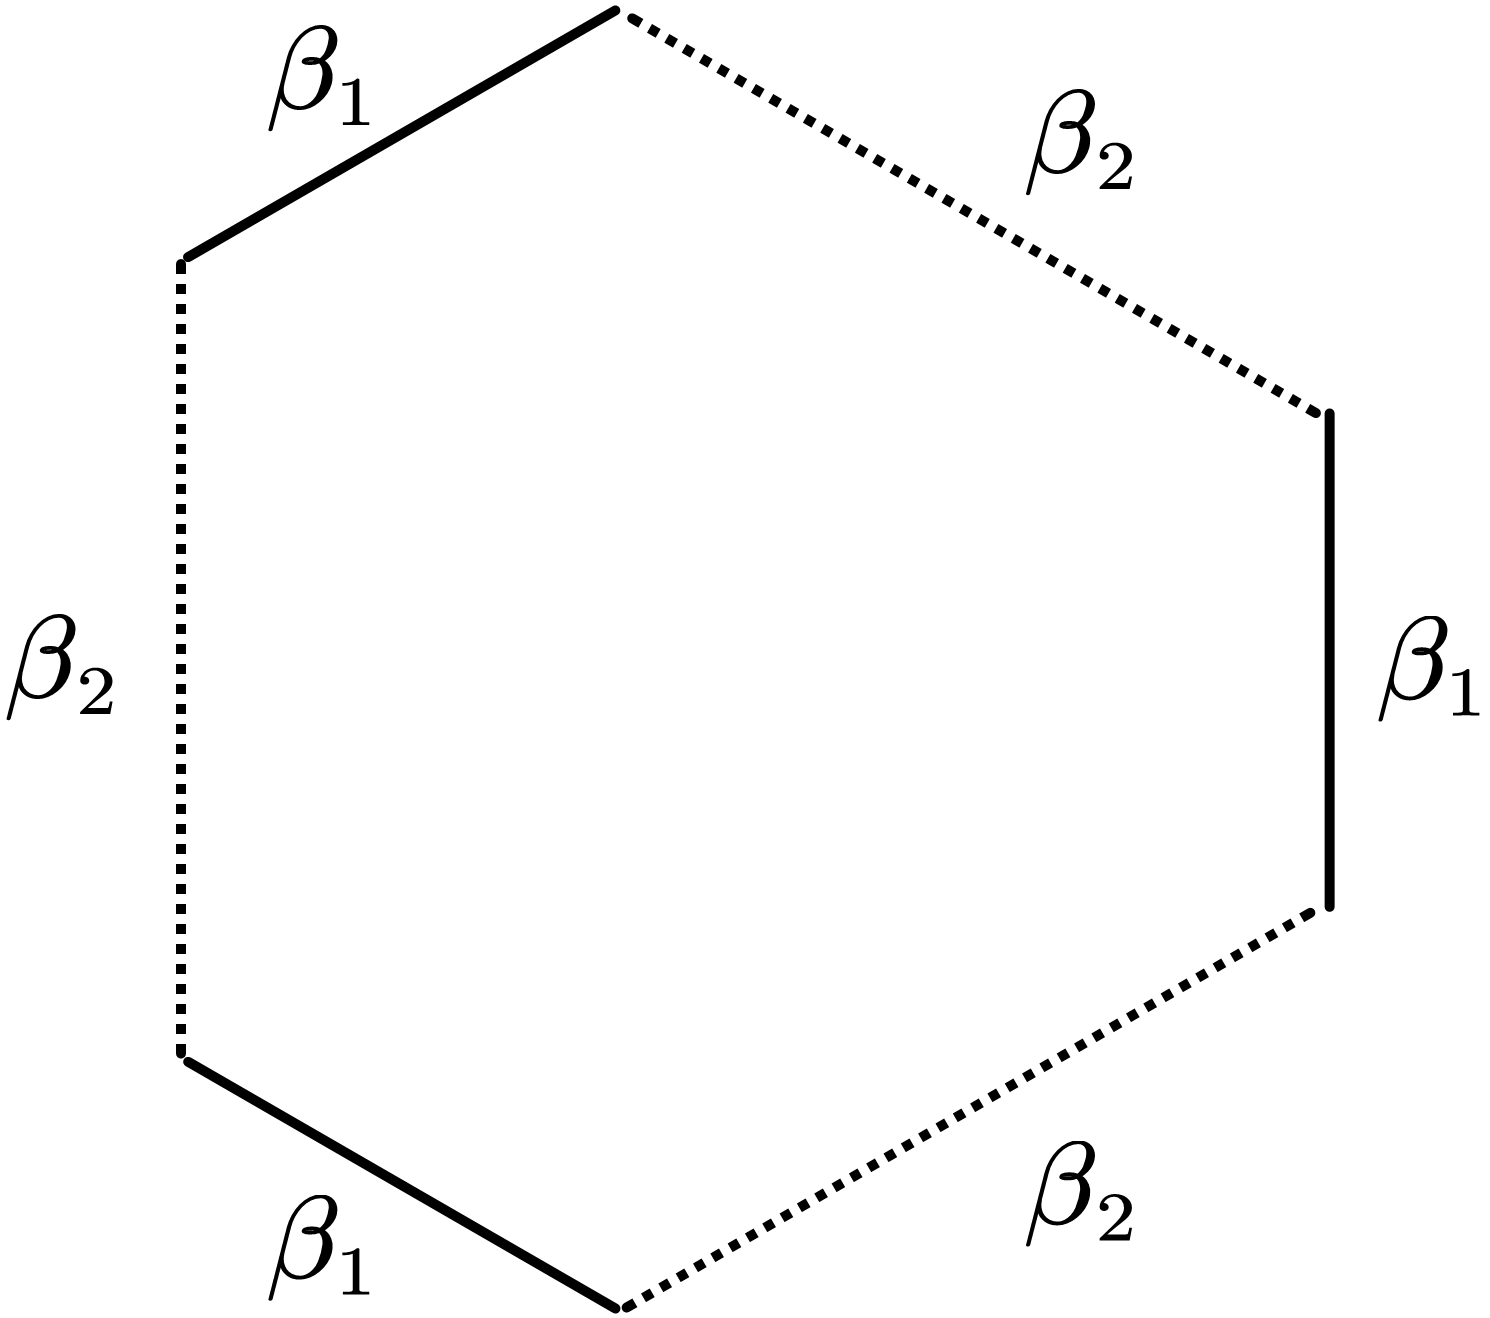
\includegraphics[scale=1.2]{./pictures/6.06/exercise_1.png}
	\end{center}
	
	Now it can be shown that the exact energy for a cyclic polyene of this type is
	\[
		\mathscr{E}_0 = N \alpha - 2 \sum_{j=-\nu}^\nu \left( \beta^2_1 + \beta^2_2 + 2 \beta_1 \beta_2 \cos{\frac{2j\pi}{2\nu+1}} \right)^{1/2}
	\]
	(see for example, L. Salem, {\it Molecular Orbital Theory of Conjugated Systems}, Benjamin, New York, 1966, pp.498-500). Note that when $\beta_1 = \beta_2 = \beta$, since $2\cos^2\theta=(1+\cos2\theta)$ and $\beta$ is negative, we recover
	\[
		\mathscr{E}_0 = N \alpha + 4 \beta \sum_{j=-\nu}^\nu \cos{\frac{j\pi}{2\nu+1}}
	\]
	which is the result quoted in Subsection 5.3.2. Also note that when $\beta_1=\beta$ but $\beta_2=0$, we have
	\[
		\mathscr{E}_0 = N \alpha + N \beta
	\]
	which is just the total energy of the polyene using the localized ethylenic description. The purpose of this exercise is to obtain the perturbation expansion for the resonance energy by expanding the exact energy in powers of $\beta_2/\beta_1$.
	\begin{enumerate}
	
	\item[a.] Show that for benzene ($\nu=1$) the exact ground state energy in the alternating short and long bond model is
	\[
		\mathscr{E}_0 = 6 \alpha + 2(\beta_1 + \beta_2) - 4 ( \beta^2_1 + \beta^2_2 - \beta_1 \beta_2 )^{1/2}
	\]
	Do this first by using the general expression and then by setting up the H{\"u}ckel matrix, diagonalizing it and adding up the occupied orbital energies. Note that when $\beta_1=\beta_2=\beta$ we recover our old result, $6\alpha+8\beta$.
	
	\item[b.] Setting $\beta_1 = \beta$ and $\beta_2/\beta_1=x$ show that the resonance energy of benzene can be written as
	\[
		E_R = 4 \beta ( \frac{1}{2}x - 1 + (1-x+x^2)^{1/2})
	\]
	Note that when $x=0$, $E_R=0$ and when $x=1$, $E_R=2\beta$ which is exact.
	
	\item[c.] Using the relation
	\[
		(1 + y)^{1/2} = 1 + \frac{1}{2} y - \frac{1}{8}y^2 + \frac{1}{16} y^3 - \frac{5}{128}y^4 + \cdots , \quad |y|<1
	\]	
	expand $E_R$ to fourth order in x and thus show that
	\[
		E_R = \beta ( \frac{3}{2}x^2 + \frac{3}{4} x^3 + \frac{3}{32}x^4 + \cdots )
	\]
	Identifying the coefficient of $x^n$ with the $n$th-order perturbation result (i.e., $E^(n)_0$), we have
	\begin{align*}
		E^{(2)}_0 &= \frac{3}{2} \beta, \\
		E^{(3)}_0 &= \frac{3}{4} \beta, \\
		E^{(4)}_0 &= \frac{3}{32} \beta.
	\end{align*}
	Note that $E^{(2)}_0$ and $E^{(3)}_0$ agree with our previously calculated values. This derivation provides some insight into the poor convergence of the perturbation expansion of the resonance energy of benzene. Basically, the perturbation expansion converges rapidly when $x$ is small. However, for our problem $x$ is equal to unity.
	
	The resonance energy calculated up to $M$th-order as a function of $M$ is shown below. Note the oscillatory convergence towards the exact value to $2\beta$. The method used above to obtain $E^{(n)}_0$ for $n=2,3,4$ becomes extremely laborious for larger $n$. The results below were calculated by first showing that $E^{(n)}_0 = 4\beta C^{-1/2}_n(1/2)$, where $C^{-1/2}_n(x)$ is a Gegenbauer polynomial of degree $n$ and order $-\frac{1}{2}$, and then using the recursive properties of these polynomials, to show that
	\[
		(n+1)E^{(n+1)}_0 = (n-1) E^{(n)}_0 - (n-2) E^{(n-1)}_0.
	\]
	
	\begin{center}
	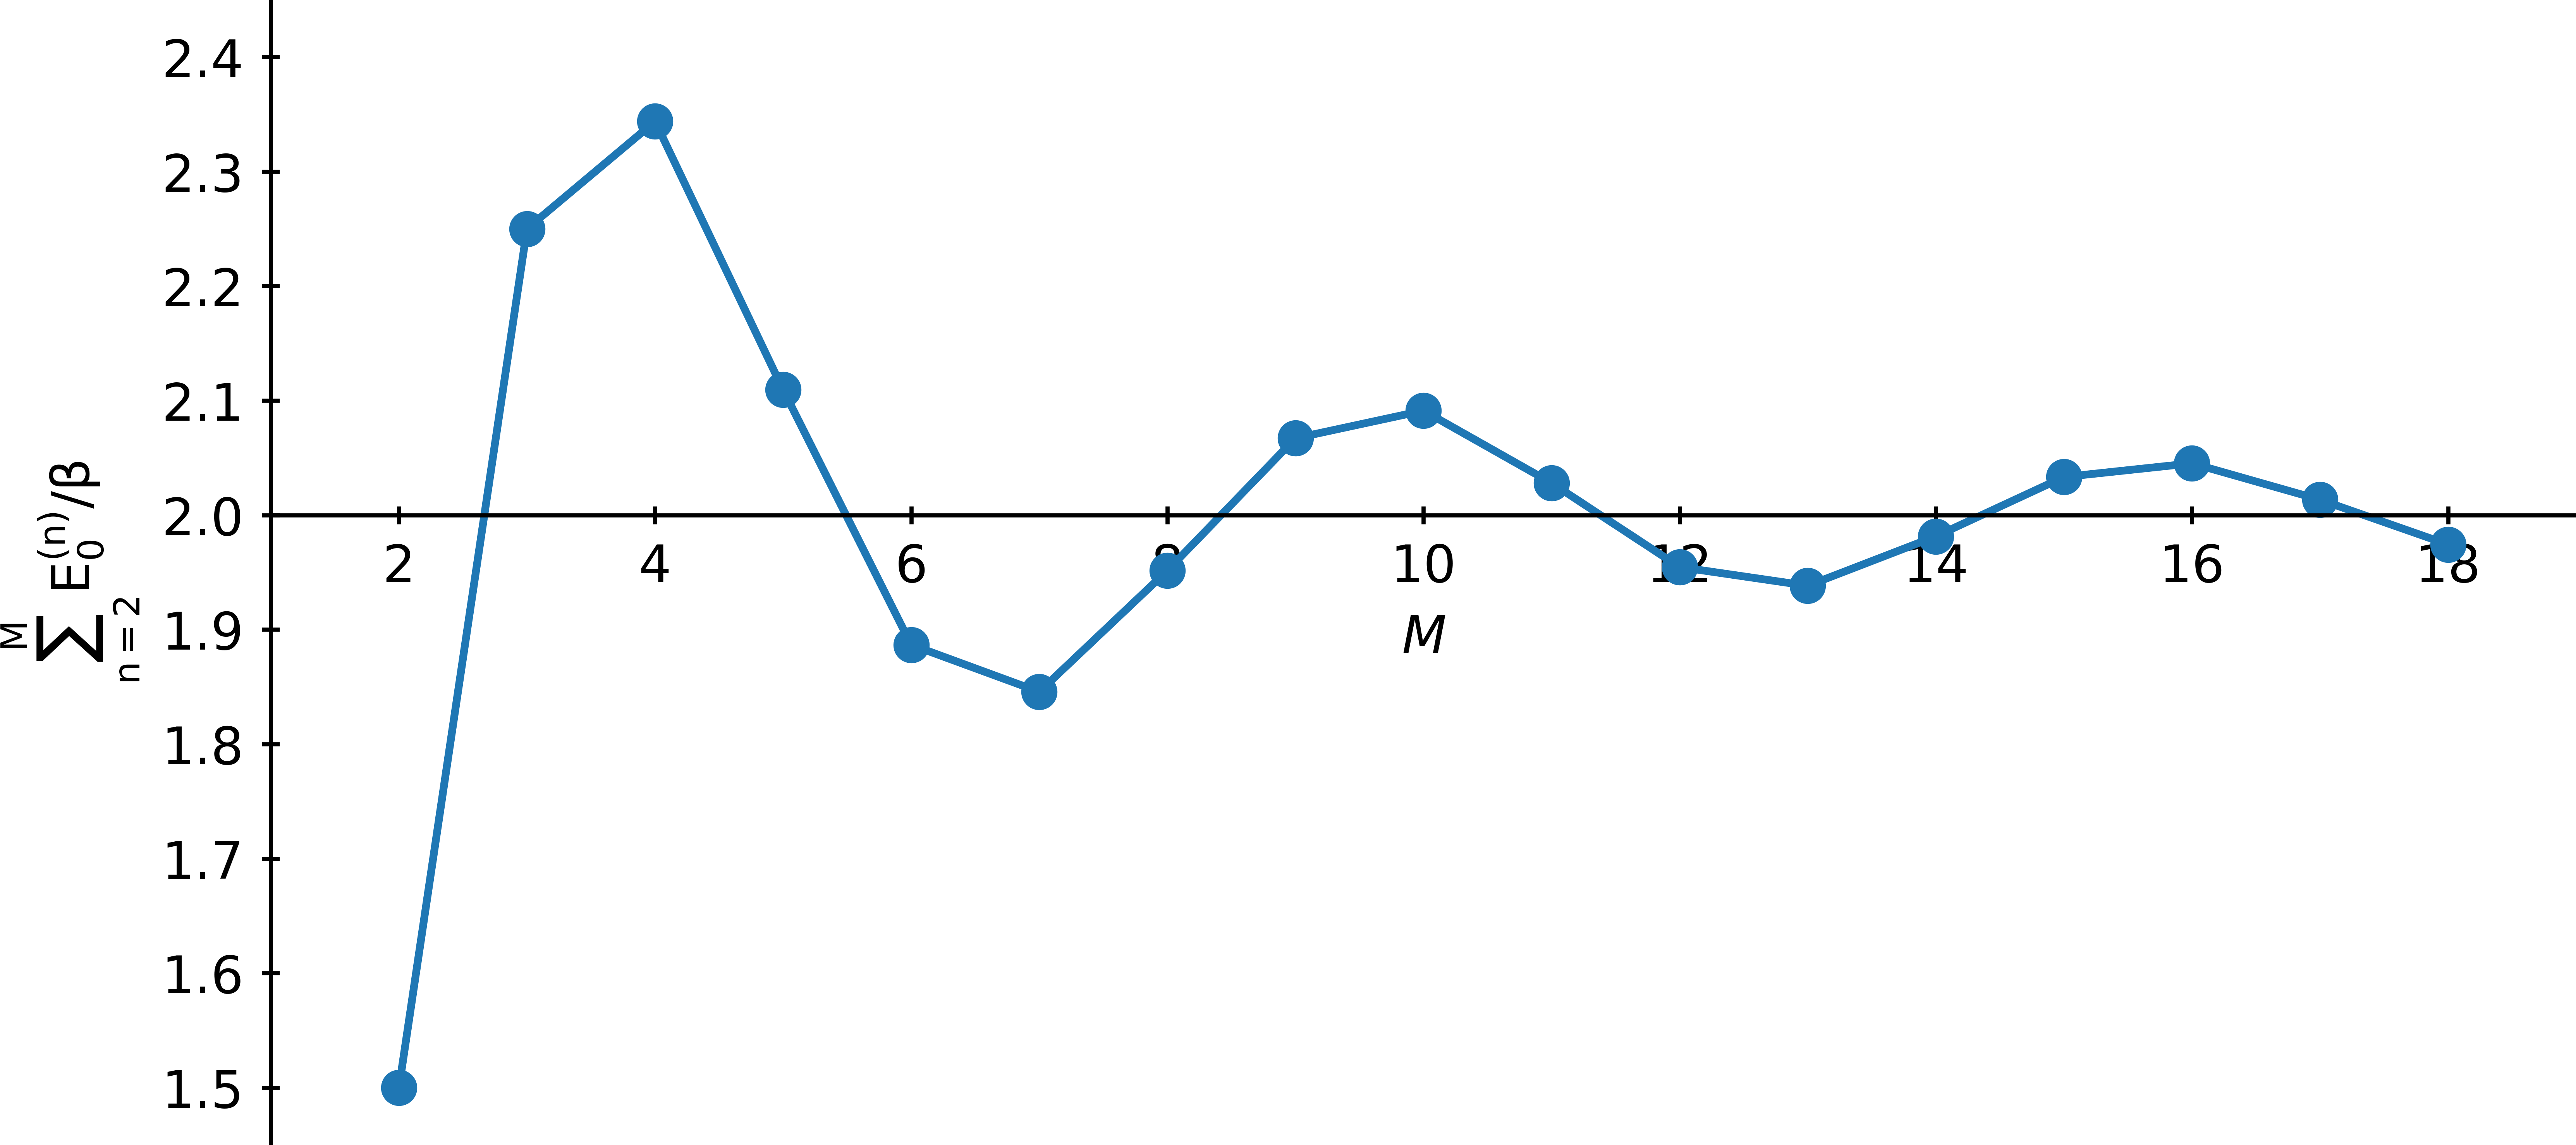
\includegraphics[scale=0.8]{./pictures/6.06/gegenbauer.png}
	\end{center}
	
	\end{enumerate}
	
	\end{exercise}
	
	\begin{solution}
		6-6 so
		
		ffff
		
		ffff
		
		fffff
		
	\end{solution}
	
	\section{Diagrammatic Representation of Orbital Perturbation Theory}
	

\end{document}
